%%This is a very basic article template.
%%There is just one section and two subsections.
\documentclass[a4paper]{article}

% acronyms
\usepackage{xspace}
\def\FFD{\emph{FFD}\xspace}
\def\WFD{\emph{WFD}\xspace}
\def\WFDINC{\emph{WFD-INC}\xspace}
\def\WFDIP{\emph{WFD-IP}\xspace}
\def\SOTA{\emph{SOTA}\xspace}
\def\BFS{\emph{BFS}\xspace}
\def\openspace{\emph{open-space}\xspace}
\def\mapevent{map-event}
\def\runtime{run-time}
\def\MyTikzScale{1.7}

\usepackage{fullpage}

%graphics
\usepackage{graphicx}
\usepackage{subfigure}

%algorithms
\usepackage[section]{algorithm}
\usepackage{algpseudocode}
\renewcommand{\algorithmiccomment}[1]{// #1}

%math
\usepackage{amsmath}
\usepackage{amssymb,latexsym}
\usepackage{amsthm}

%theorems
\newtheorem{theorem}{Theorem}[section]
\newtheorem{lemma}[theorem]{Lemma}
\newtheorem{proposition}[theorem]{Proposition}
\newtheorem{corollary}[theorem]{Corollary}

%environments
\newenvironment{definition}[1][Definition.]{\begin{trivlist}
\item[\hskip \labelsep {\bfseries #1}]}{\end{trivlist}}
\newenvironment{example}[1][Example.]{\begin{trivlist}
\item[\hskip \labelsep {\bfseries #1}]}{\end{trivlist}}
\newenvironment{remark}[1][Remark]{\begin{trivlist}
\item[\hskip \labelsep {\bfseries #1}]}{\end{trivlist}}
\newenvironment{proofsketch}[1][Proof Sketch]{\begin{trivlist}
\item[\hskip \labelsep {\bfseries #1}]}{\end{trivlist}}
% \newenvironment{proof}[1][Proof]{\begin{trivlist}
% \item[\hskip \labelsep {\bfseries #1}]}{\end{trivlist}}

\usepackage{verbatim}

%%% shortcuts
\newcommand{\term}[1]{{\left(#1\right)}}
\newcommand{\execTime}[1]{#1^\term{t}}
\newcommand{\order}[1]{\mathcal{O}\term{#1}}

% tikz drawings
\usepackage[usenames,dvipsnames]{xcolor}
\usepackage{tikz}
\usetikzlibrary{matrix,arrows}

\begin{document}

\title{Efficient Frontier Detection for Robot Exploration}
\author{Matan Keidar \and Gal A. Kaminka}
\maketitle

\Abstract{ 
Frontier-based exploration is the most common approach to exploration, a
fundamental problem in robotics. In frontier-based exploration, robots
explore by repeatedly computing (and moving towards) \emph{frontiers},
the segments which separate the known regions from those unknown. However, most
frontier detection algorithms process the entire map data. This can be a time
consuming process which slows down the exploration. In this thesis, we present
two novel frontier detection algorithms: \WFD, a graph search based
algorithm and \FFD, which is based on processing only the
new laser readings data. In contrast to state-of-the-art methods, both
algorithms do not process the entire map data. 
This thesis contains a theoretical complexity analysis for both algorithms and
since \FFD is a novel approach, we proove its correctness. We succeeded to
improve \WFD and \FFD performance even further by combining them into two new algorithms called \WFDINC and \WFDIP.
We implemented all algorithms and showed that all are faster than a
state-of-the-art frontier detector implementation (by several orders of magnitude).
}


\section{Introduction}
\label{chap:introduction}
The problem of exploring an unknown territory is a fundamental problem in
robotics. The goal of exploration is to gain as much information as possible
of the environment within bounded time. 
Applications of efficient exploration include search and rescue \cite{Kitano99robocuprescue}, planetary exploration \cite{apostolopoulos2001robotic} and military uses \cite{hougen2000miniature}.
The most common approach to exploration is based on \emph{frontiers}. A frontier
is a segment that separates known (explored) regions from unknown regions. By
moving towards frontiers, robots can focus their motion on discovery of new
regions. Yamauchi
\cite{yamauchi_frontier-based_1997,yamauchi_frontier-based_1998} was the first
to show a frontier-based exploration strategy. His work led to many
others (e.g,
\cite{burgard05tro,lau_behavioural_2003,sawhney_fast_2009,burgard_collaborative_2000}).

Most frontier detection methods are based on edge detection and region
extraction techniques from computer vision. To detect frontiers, they
process the entire map data with every execution to the algorithm.
State-of-the-art frontier detection algorithms can take a number of seconds to run, even on powerful
computers. If a large region is explored, the robot actually has to wait in its
spot until the frontier detection algorithm terminates. Therefore, many
exploration implementations call the frontier detection algorithm only when the
robot arrives at its destination. 
 
This slows down the exploration process. It also can cause inefficiencies in the
exploration.
We present two examples:
First, consider a common \textit{single-robot case} (Figure~\ref{fig:single_example}),
where a robot exploring its environment detects a frontier and moves towards it (Figure~\ref{fig:single_1}).
Because of sensor coverage, the robot may in fact sense (and clear) all remaining unknown
area (Figure~\ref{fig:single_2}), but because it cannot call the
frontier-detection mechanism, it continues to move unnecessarily
(Figure~\ref{fig:single_3}). Similarly, consider a \textit{multi-robot case}
(Figure~\ref{fig:mutli_example}). Here, two robots,
 $R_1$ and $R_2$ which are located on bottom and top, respectively, 
are exploring the environment, from their initial locations (Figure~\ref{fig:multi_1}). 
One of the robots passes by a target assigned to the other, and thus clearing it
(Figure~\ref{fig:multi_2}).
But because the other robot cannot continuously re-detect frontiers, it unnecessarily continues
towards the covered target, instead of turning to more fruitful exploration targets.

\begin{figure}
 \centering
 \subfigure[ ] {
 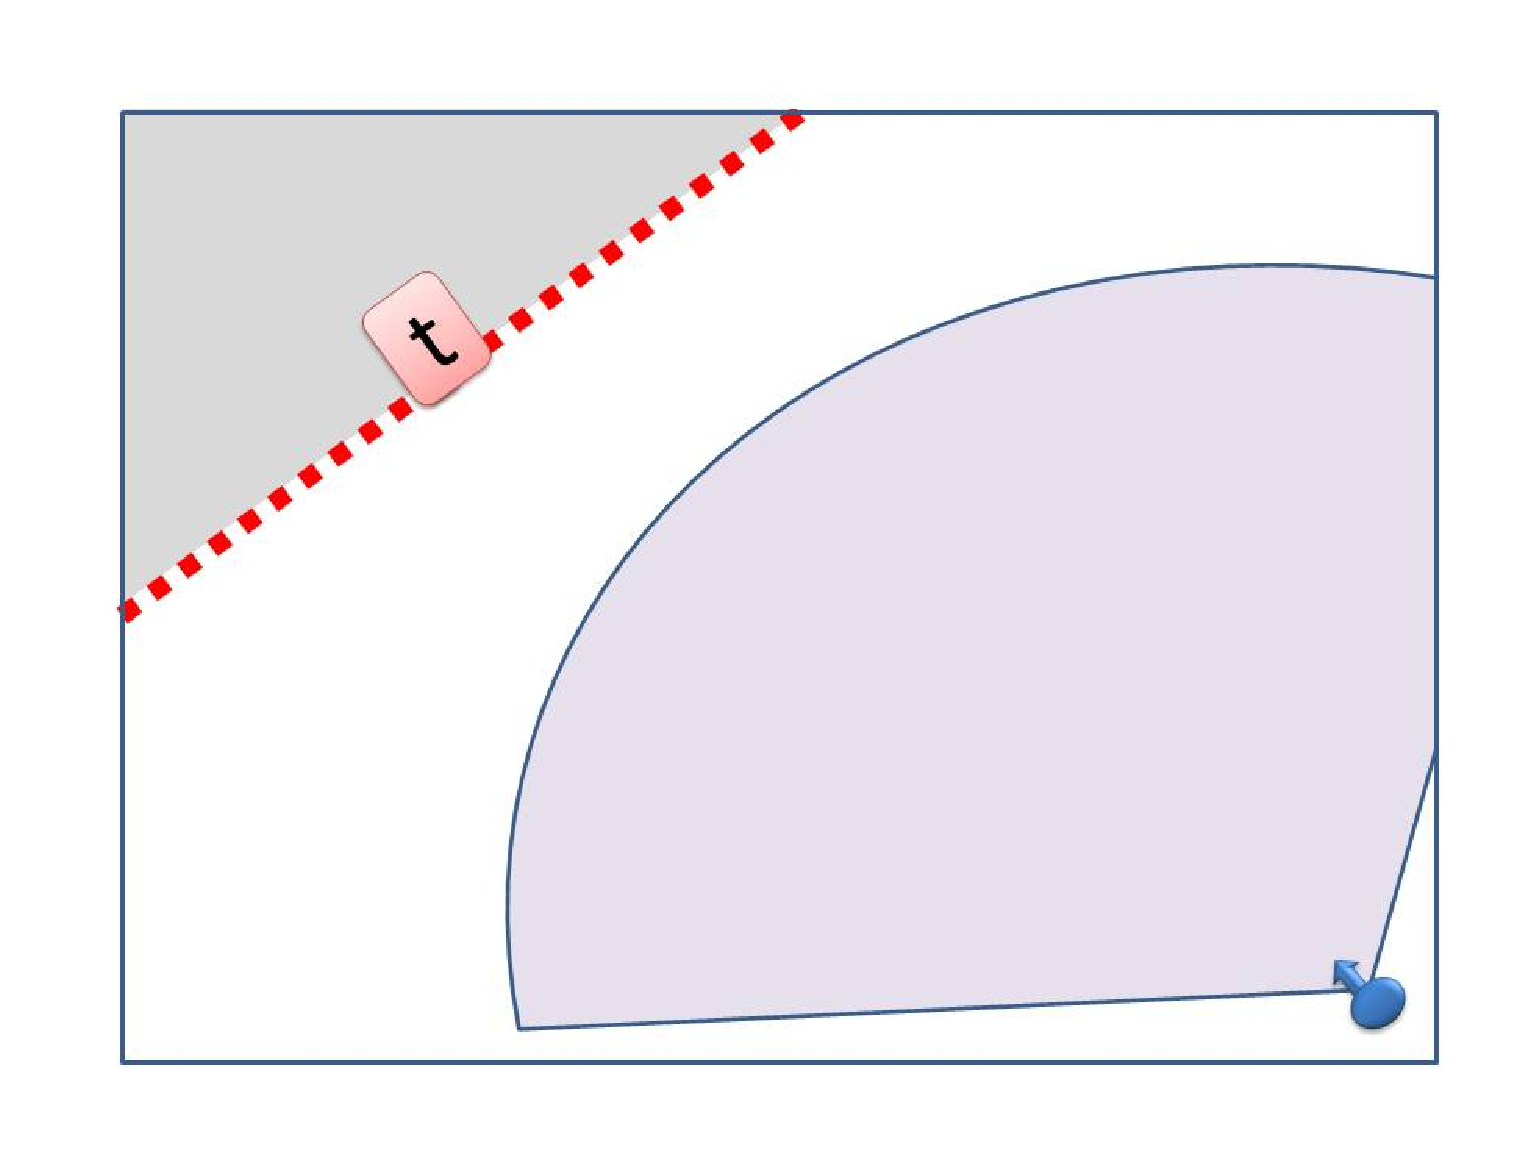
\includegraphics[width=0.3\columnwidth,keepaspectratio]{images/single_1}
 \label{fig:single_1}}
 \subfigure[ ] {
 \centering
 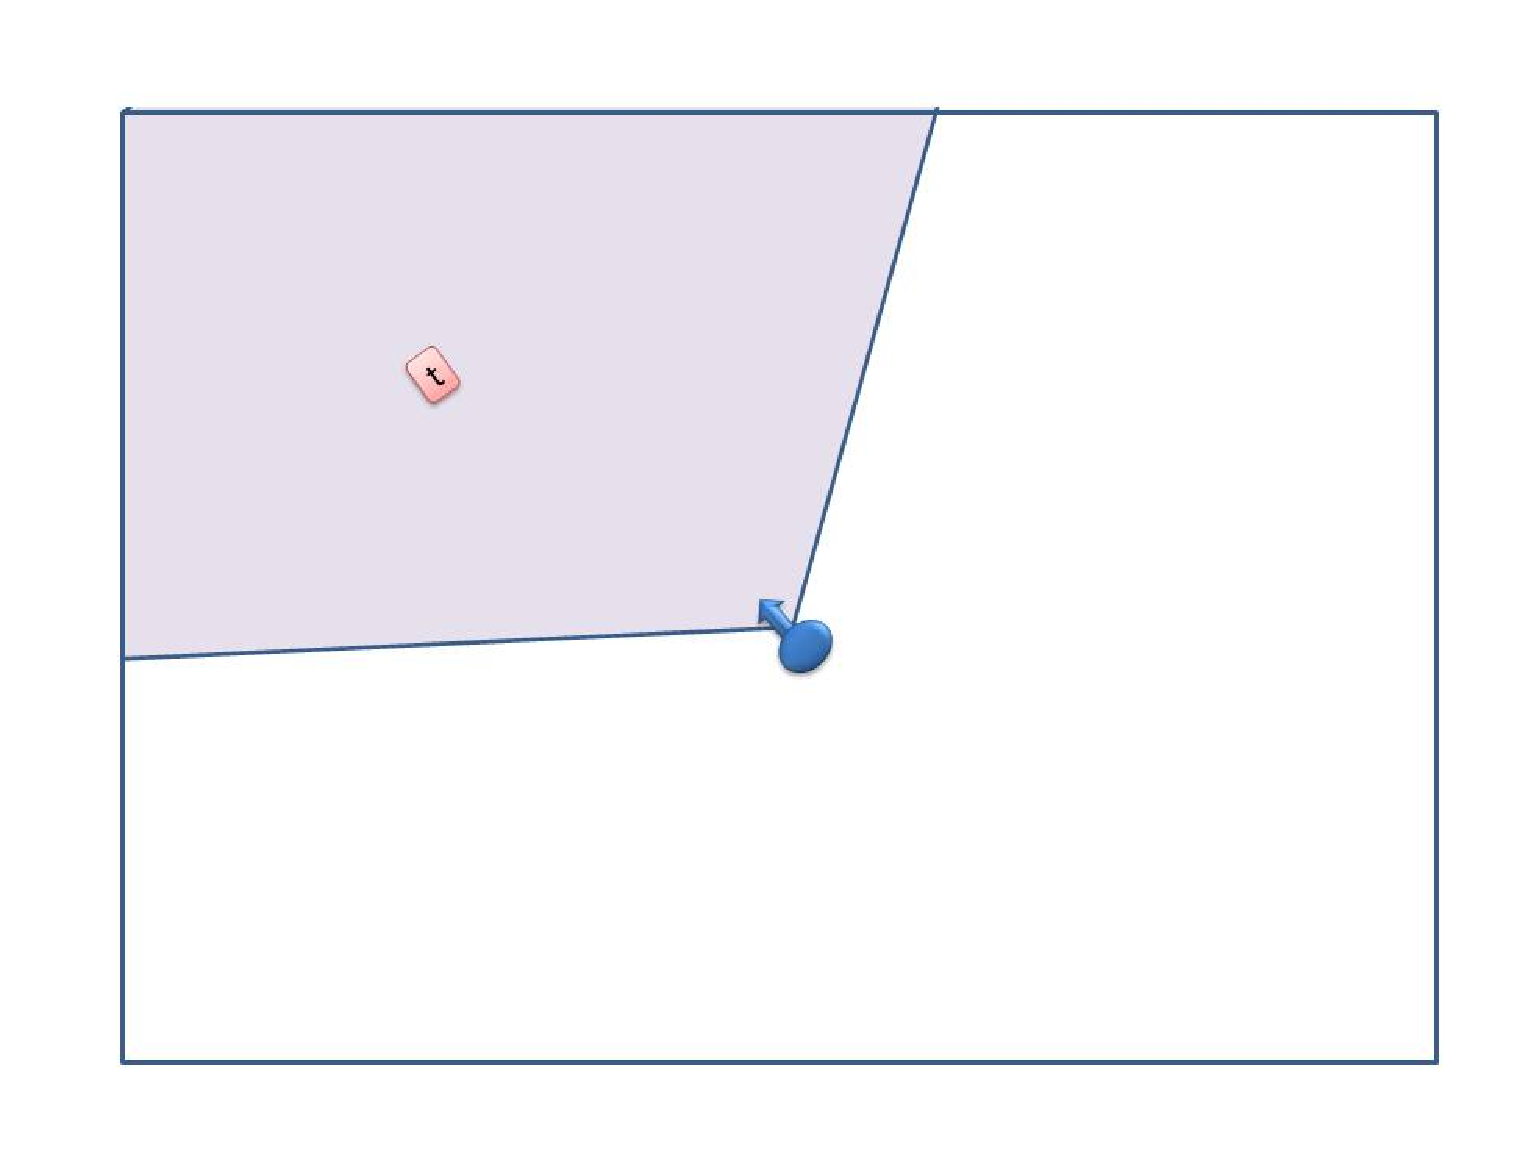
\includegraphics[width=0.3\columnwidth,keepaspectratio]{images/single_2}
 \label{fig:single_2}}
 \subfigure[ ] {
 \centering
 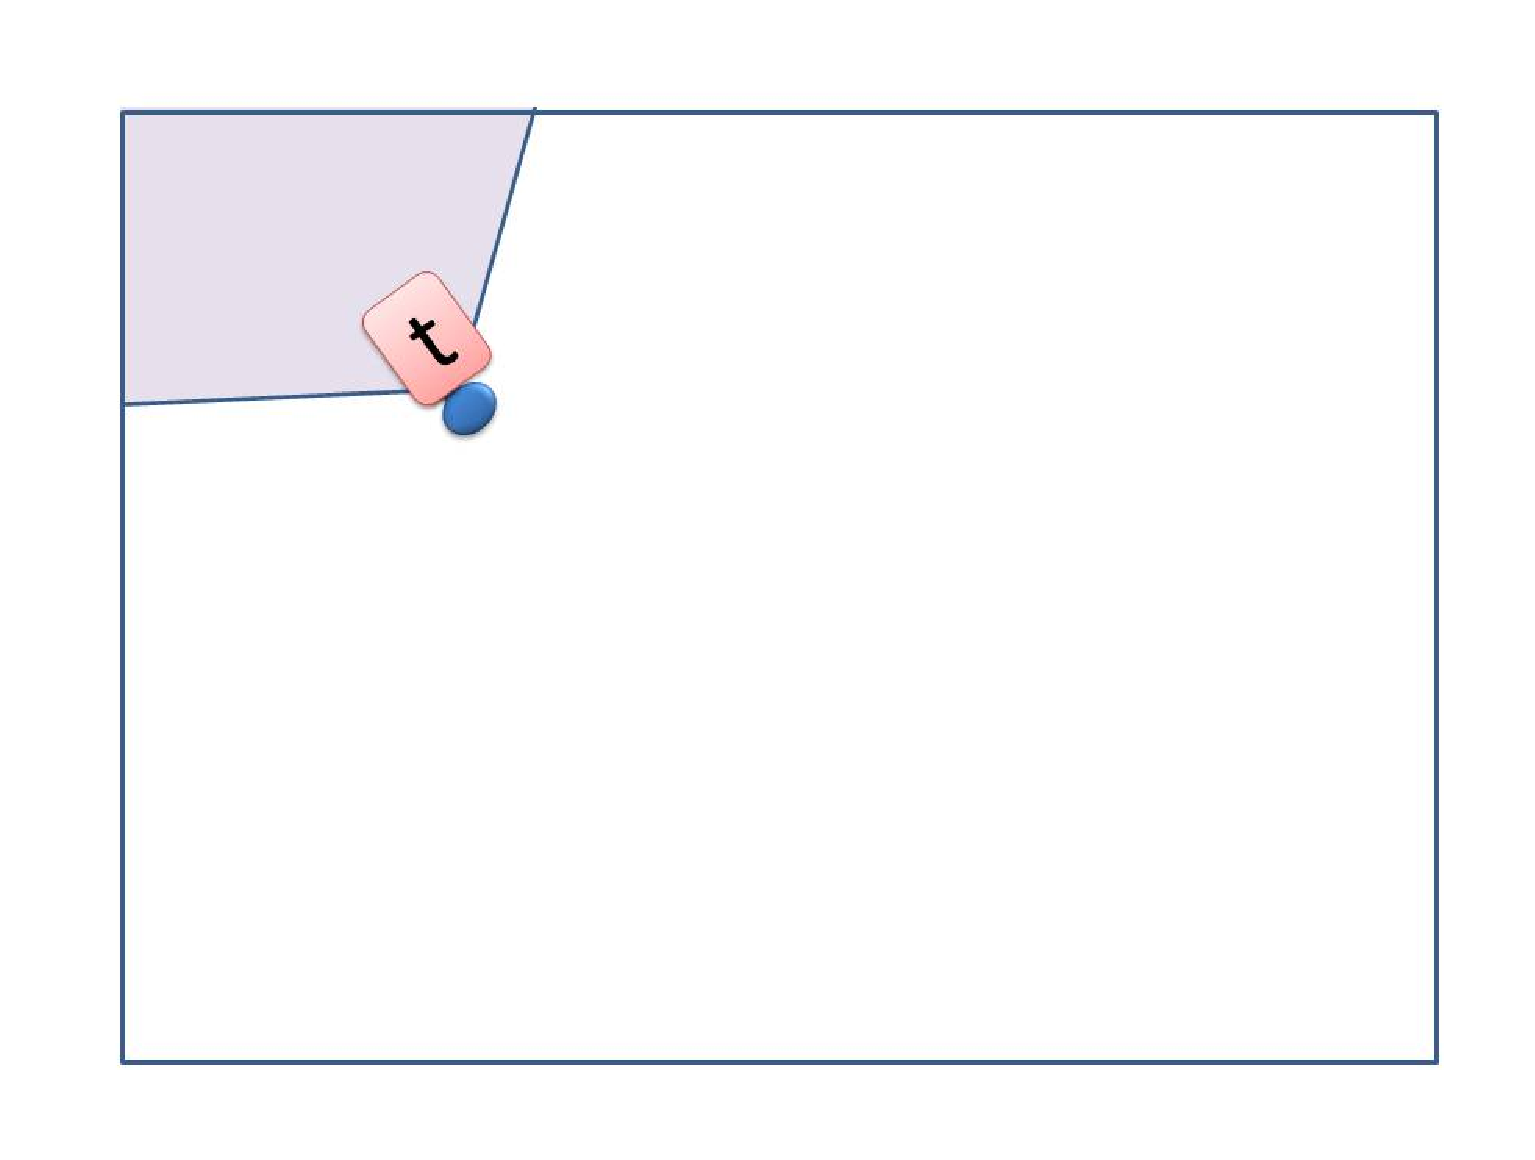
\includegraphics[width=0.3\columnwidth,keepaspectratio]{images/single_3}
 \label{fig:single_3}
 }
 \caption{A single-robot example. In 
 \ref{fig:single_1} the robot is heading towards the marked target on the frontier.  In 
 \ref{fig:single_2} the target and all of the remaining are covered by the robot's sensors, but because the robot does
  not re-detect frontiers, it continues to move.  In  \ref{fig:single_3} the robot has reached the frontier, unnecessarily.
 }
 \label{fig:single_example}
 
\end{figure}


\begin{figure}
 \centering
 \subfigure[] {
 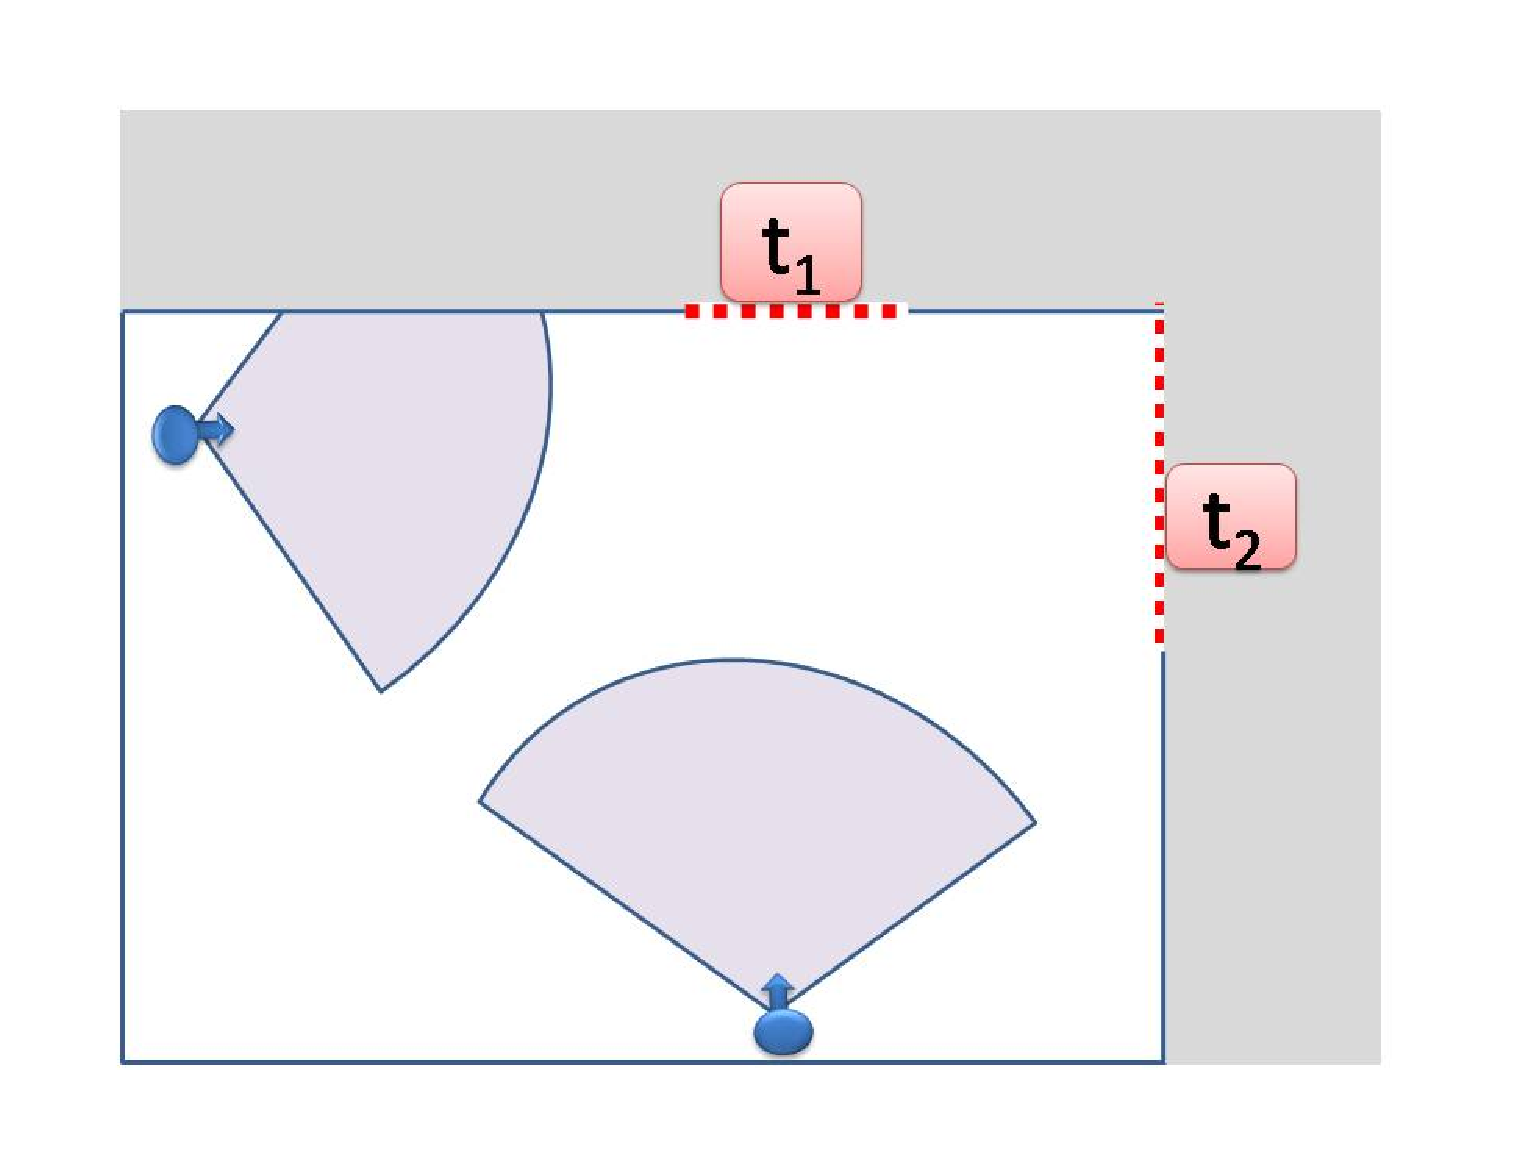
\includegraphics[width=0.45\columnwidth,keepaspectratio]{images/multi_1}
 \label{fig:multi_1}}
 \subfigure[] {
 \centering
 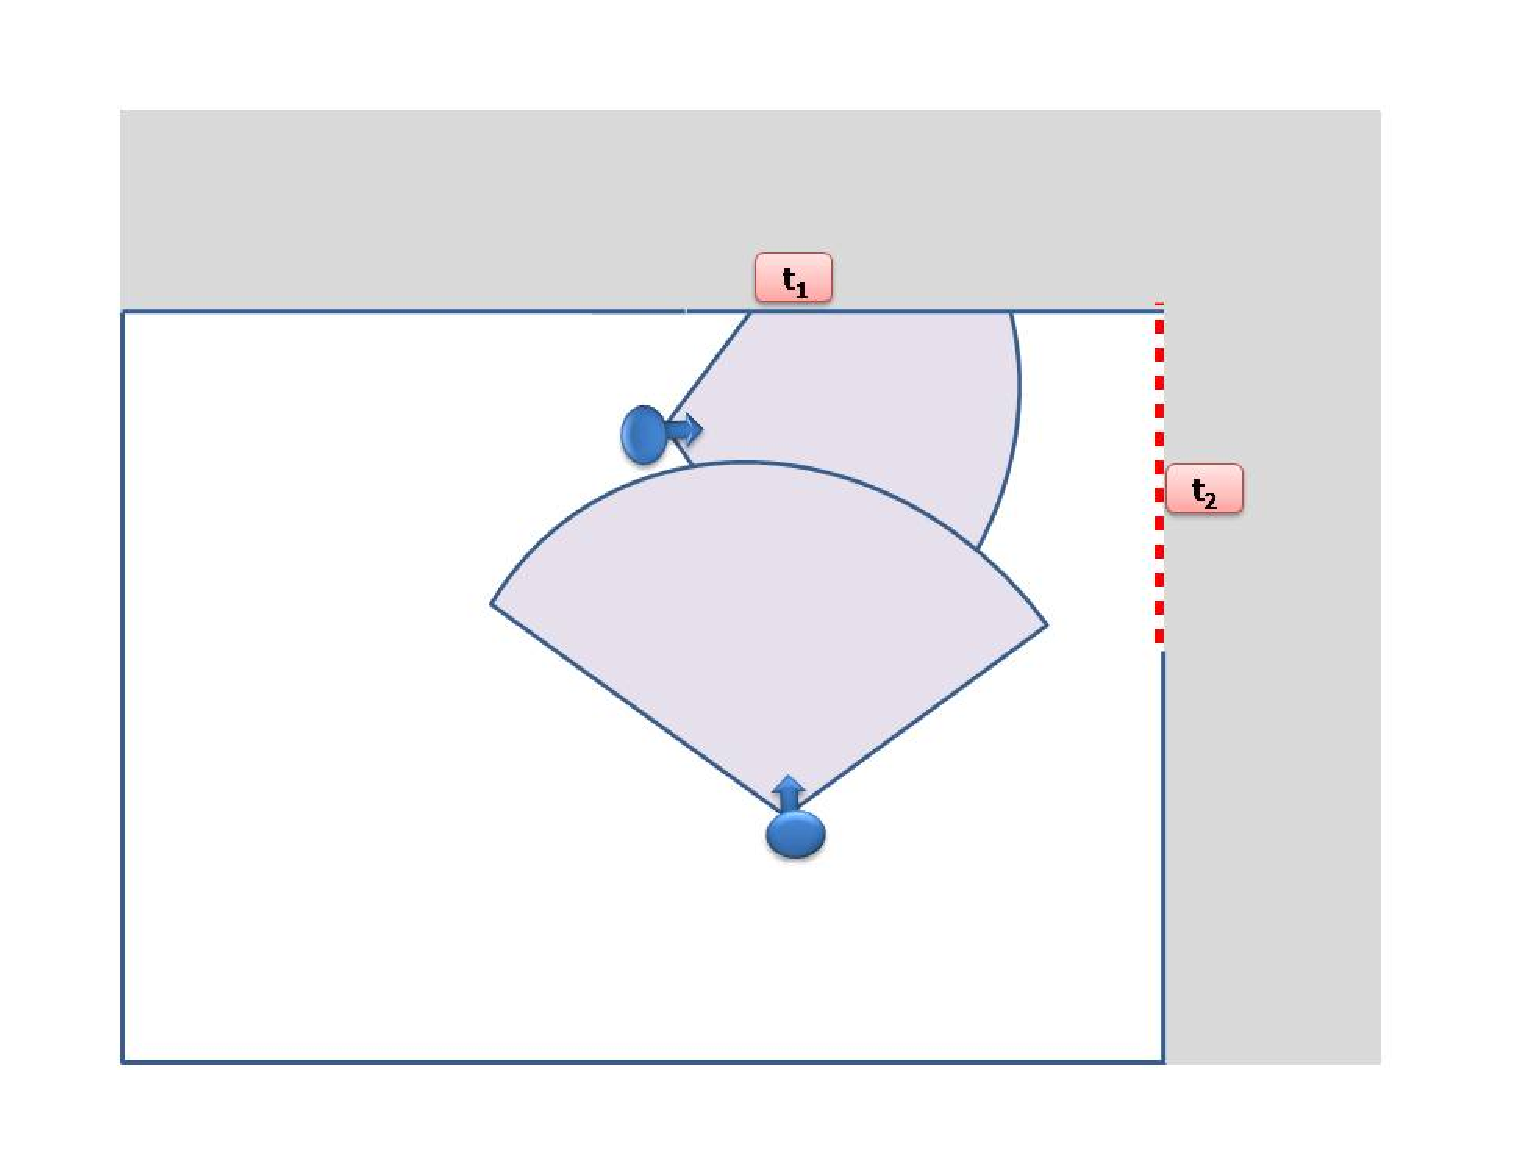
\includegraphics[width=0.45\columnwidth,keepaspectratio]{images/multi_2}
 \label{fig:multi_2}}
 \caption{A multi-robot example.  In~\ref{fig:multi_1}, the top robot ($R_2$) is heading towards the right target, $t_2$; the other robot ($R_1$) heads towards the top target $t_1$. In~\ref{fig:multi_2} $R_2$ has reached its target, clearing both $t_1$ and $t_2$, making $R_1$'s movements unnecessary.}
 \label{fig:mutli_example}
\end{figure}

In this thesis, we thus focus on significantly speeding up frontier detection.
We introduce four algorithms for fast frontier detection: 
The first, \WFD (Wavefront Frontier Detector) % (Section \ref{section:wfd})
is an iterative method that performs a graph-search over already-visited map
points. It builds on ideas suggested in earlier
work~\cite{Calisi:2007:MES:1291068.1291076} which were not evaluated as an
alternative to the edge-detection state-of-the-art. The key idea in \WFD is
that it does not scan the entire map, only the regions that have already been
visited by the robot.
However, as exploration progresses, the scanned area grows, and thus \WFD cannot
be expected to perform well in large areas.  Our second contribution is 
\FFD (Fast Frontier Detector), % (Section \ref{section:ffd}) is 
a novel approach for frontier detection which processes raw sensor readings,
and thus only scans areas that could contain frontiers. But because it works
with raw sensor data, it requires extending the mapper (SLAM) with additional
data-structures, so that frontiers are maintained
even when they are no longer within sensor range.
We describe these data-structures in detail, focusing on 
fast implementations.
Finally, we synthesized the different approaches of
\WFD and \FFD into two novel algorithms: \WFDINC and \WFDIP. Both algorithms
perform frontier detection on known regions but they differ from \WFD by
searching for frontiers only within the areas that were covered by the robot
sensors since last call.

\WFD and edge-detection methods use the occupancy grid
maintained by a SLAM mapper as a representation of the accumulated, processed sequence $\langle
O_0,\ldots,O_t\rangle$. They thus essentially ignore most of the sequence, and
act (mostly) on the latest observation of the grid $G_t$, as it integrates all
sensor readings up to time $t$. The edge detection method processes $G_t$ (the
entire occupancy grid at time $t$). The \WFD algorithm processes a subset,
starting with the cell indicated by $P_t$ (the latest robot position), within
$G_t$.  \FFD uses $R_t$ directly to detect current frontiers, and a modified
occupancy grid data structure to maintain/delete past frontiers.
We provide a theoretical complexity analysis for both algorithms and
in addition, \FFD is a novel approach and hence we proove its correctness. 
More definitions and terms related to the frontier detection problem can be
found in Section \ref{section:definitions}.

We provide a detailed evaluation of these algorithms, and contrast them 
with the state-of-the-art (\SOTA). % (in Section
% \ref{section:experimental_results}.
We examine their performance in different types of environments and two different
CPUs. We show that \WFD and \WFDINC are faster than \SOTA by 1--2 orders of
magnitude, and that \FFD and \WFDIP are faster than \WFD and \WFDINC by 1--2
orders of magnitude.  The results make it possible to execute real-time
frontier-detection on current-day robot CPUs, opening the way to novel
frontier-based exploration methods which were impractical until now.

\paragraph{List of Publications}
The work reported in this thesis has been published in the following
conferences:
\begin{itemize}
  \item \nobibentry{keidar2011arms}
  \item \nobibentry{keidar2012aamas}
\end{itemize}

This paper is organized as follows. Section~\ref{chap:related_work} discusses
related investigations. Sections~\ref{chap:wfd}~and~\ref{chap:ffd} discuss 
the \WFD and \FFD algorithms, respectively, including their theoretical
correctness. Section~\ref{chap:complexity}
discusses  complexity of these methods. 
Section~\ref{chap:maint} shows how to combine elements of \WFD and \FFD
to create two improved algorithms, \WFDINC and \WFDIP. Section~\ref{chap:results}
reports on empirical evaluation of all algorithms, contrasting with the
state of the art. Finally, Section~\ref{chap:conclusions} concludes.

\section{Related Work}
\label{chap:related_work}
\input{related_work}

\section{Wavefront Frontier Detector}
\label{chap:wfd}
In this section we review the basic definitions and terms related to the domain
of frontier-based exploration, as well as a formal definition of the
frontier-based exploration problem (Section~\ref{section:definitions}). We briefly discuss
common state-of-the-art techniques for performing a Simultaneous
Localization and Mapping (Section~\ref{section:slam}), which underly existing
approaches to exploration. We then present the \WFD algorithm
which searches for frontiers on the map (Section~\ref{section:wfd}).

\subsection{Frontier-Based Exploration: Definitions}
\label{section:definitions}
In this section we define and explain the terms that are used in the following
sections. We assume the robot in question uses an occupancy-grid map
representation in the exploration process (Figure \ref{fig:frontiers}) within the map:

\noindent{\bf Unknown Region} is a territory that has not been covered yet by
the robot's sensors.
	
\noindent{\bf Known Region} is a territory that has already been covered by the
robot's sensors.
	
\noindent{\bf Open-Space} is a \emph{known region} which does not contain an
obstacle.

\noindent{\bf Occupied-Space} is a \emph{known region} which contains an
obstacle.

\noindent{\bf Occupancy Grid} is a grid representation of the environment. Each
cell holds a probability that represents if it is occupied.

\noindent{\bf Frontier} is the segment that separates known (explored) regions
from unknown regions. Formally, a frontier is a set of \emph{unknown} points that each have at
least one \emph{open-space} neighbor.

\begin{definition}
Suppose we are given a temporal sequence of observations $\langle
O_0,\ldots,O_t\rangle$ (time 0 to time $t$), where each observation $O_x$ is a
tuple $\langle G_x, P_x, R_x\rangle$ composed of: (i) the occupancy-grid $G_x$
of time $x$; (ii) the robot pose $P_x$ (in occupancy-grid coordinates); and
(iii) the range sensor readings $R_x$ originating at the robot location (given
in either ego-centric polar coordinates, or in occupancy-grid coordinates).
The \emph{Frontier Detection Problem} is to return all frontiers existing at
time $t$, given the sequence.
\end{definition}


% \begin{figure}
%  \centering
%  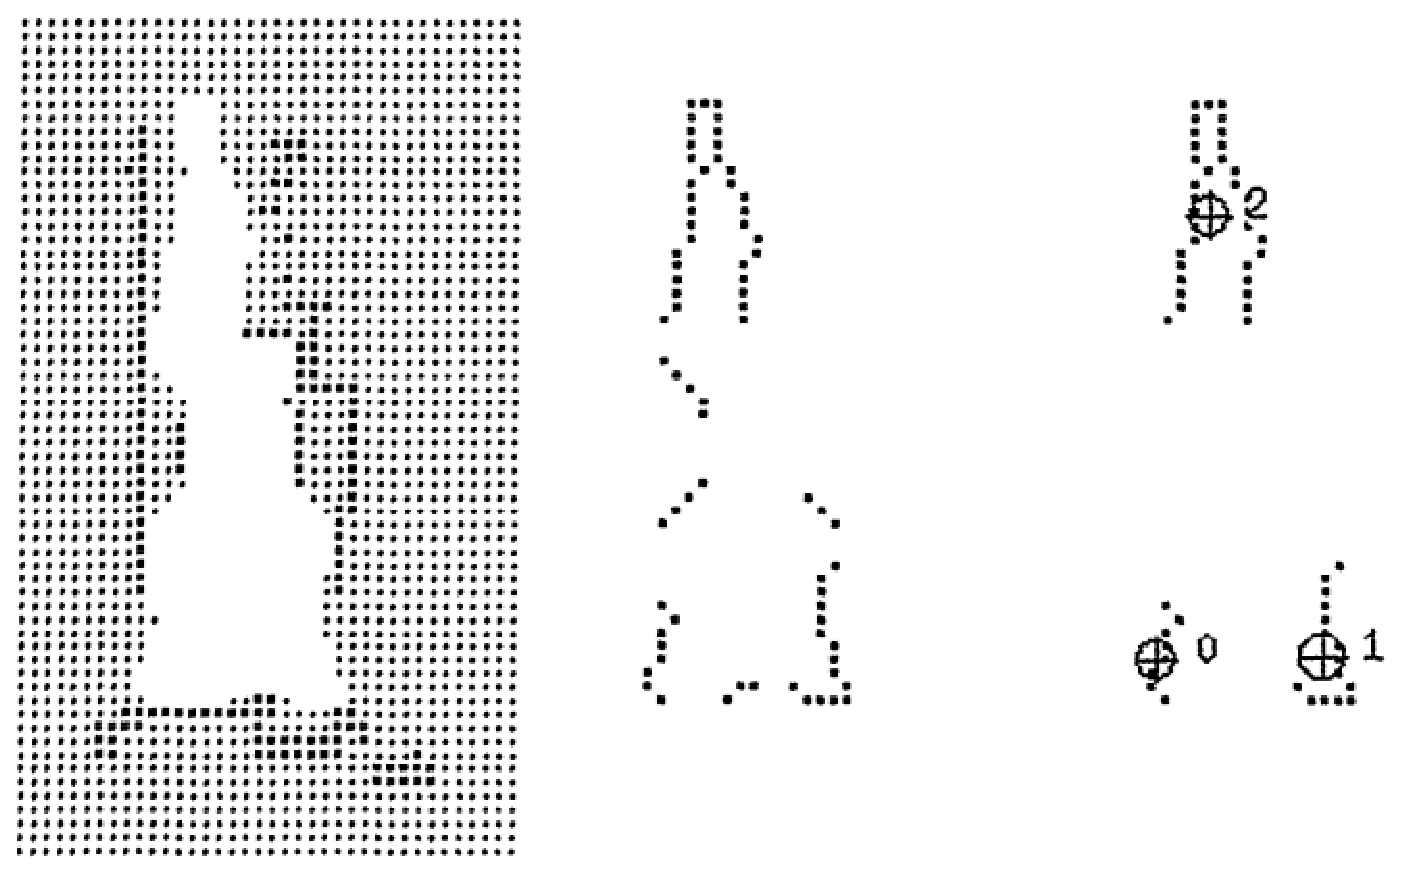
\includegraphics[width=0.8\columnwidth,keepaspectratio]{frontiers_example}
%  \caption{Evidence grid, frontier points, extraction of different frontiers (from left to
%  right). Taken from \protect\cite{yamauchi_frontier-based_1998}.}
%  \label{fig:frontiers}
% \end{figure}

\begin{figure}
 \centering
 
\includegraphics[width=0.5\columnwidth,keepaspectratio]{octave/frontiers_combined_fixed}
 \caption{Evidence grid, frontier points (from left to
 right).}
 \label{fig:frontiers}
\end{figure}

Existing algorithms for frontier detection rely on edge-detection methods. The
algorithms systematically search for frontiers all over the occupancy-grid,
i.e., both in known and unknown regions.

\subsection{Simultaneous Localization and Mapping Methods}
\label{section:slam}
Simultaneous Localization and Mapping (\emph{SLAM}) is a method utilized by
autonomous mobile robots for building a map of an unknown environment while at
the same time navigating the environment using the map. The term \emph{SLAM} was
originally developed by Leonard et al. \cite{leonard1991mobile,durrant2006simultaneous}.
In \emph{SLAM} both the trajectory of the mobile robot,
its location and the location of the landmarks observed by the robot are
estimated without using any \emph{a priori} knowledge of the environment.
\emph{SLAM} is a concept and hence, there are various algorithms in literature
which deal with the \emph{SLAM} problem:  

\paragraph{Extended Kalman Filter}
The \emph{Kalman Filter} (\emph{KF}) is a method for implementing Bayes
filters.
It was invented by Rudolph Emil Kalman \cite{welch1995introduction,
Thrun2005Probablistic} to apply filtering and perform prediction in linear
systems. In Kalman Filter, beliefs are represented by moments (i.e., by the mean
and the covariance). Markov assumptions are held and the posteriors are
Gaussian. Kalman filters are based on \emph{linear} system dynamics. However,
real-world systems are seldom linear in practice (e.g., robot which moves in a
cyclic path). The \emph{Extended Kalman Filter} (\emph{EKF}) uses a non-linear
functions that describe the system dynamics. In \emph{EKF-SLAM} systems, there
is only one map (part of the system state) that is composed from the observed
landmarks.
  
\paragraph{Particle Filter}
A \emph{Particle Filter} (also known as \emph{sequential Monte Carlo method}) is
a model estimation method which is based on simulation. Particle Filter is the
online version of \emph{Markov chain Monte Carlo} (\emph{MCMC}) methods
\cite{HASTINGS01041970,geyer1992practical,neal1993probabilistic}.
With sufficient samples, a particle filter is often an alternative to \emph{EKF}
with the advantage that it approaches the Bayesian optimal estimate and so it
is more accurate than \emph{EKF}. Each particle is a possible hypothesis of what
is the true world state at a certain time, that is, each particle is an
instance of the system state at a certain time. By state we refer to a
collection of variables such as the map of the explored environment, the robot
position etc. 

In this work we focus on particle filter systems since in practice, they
provide more accurate results. 

\subsection{\WFD}
\label{section:wfd}
We present a graph search based approach for frontier detection. The algorithm,
\WFD (Algorithm
\ref{alg:WavefrontFrontierDetector1}--\ref{alg:WavefrontFrontierDetector2}),
processes the points on map which have already been scanned by the robot sensors
and therefore, does not always process the entire map data in each run, but
only the known regions.

\WFD (Algorithm~\ref{alg:WavefrontFrontierDetector1}) is based on
Breadth-First Search (\BFS). First, the occupancy-grid point that represents the
current robot position is enqueued into $queue_m$, a queue data-structure used to determine
the search order (Algorithm \ref{alg:WavefrontFrontierDetector1} lines
\ref{mark:wfd_stat_init}--\ref{mark:wfd_end_init}).
% \begin{algorithm}[htbp]
\caption{Wavefront Frontier Detector (WFD) Part 1}
\label{alg:WavefrontFrontierDetector1}
\begin{algorithmic}[1]



\Require{$queue_m$} \Comment{queue, used for detecting frontier points from
a given map} 
 
\Require{$queue_f$} \Comment{queue, used for extracting a frontier
from a given frontier cell} 

\Require{$pose$} \Comment{current global position of the
robot} \label{mark:end_vars_bfs}



%%%%%%%%%%%%%%%%%%%%%%%%%%%%%%%%%%%%%%%%%%%%%%%%%%%%%%%%%%%%%%%
\State{$queue_m \gets \emptyset$}
\label{mark:wfd_stat_init}
\State {ENQUEUE($queue_m$, $pose$)}
\label{mark:wfd_enqueue_robot_pos}
\State {mark $pose$ as ``Map-Open-List''} \label{mark:wfd_end_init}
\Statex{}
\While {$queue_m$ is not empty}
\label{mark:wfd_start_map_bfs}
	\State{$p \gets$ DEQUEUE($queue_m$)}
	\label{mark:wfd_dequeue_map_bfs} 
	\If{$p$ is marked as ``Map-Close-List''}
		\State{continue}
	\EndIf 
	
	\If{$p$ is a frontier point}
		
		\State{$queue_f \gets \emptyset$}
		\State{$NewFrontier \gets \emptyset$}
		\State {ENQUEUE($queue_f$, $p$)}
		\State {mark $p$ as ``Frontier-Open-List''}
		\Statex{}
		\While{$queue_f$ if not empty}
		\label{mark:wfd_start frontier_extraction_bfs}
			\State{$q \gets$ DEQUEUE($queue_f$)} 
			\label{mark:wfd_dequeue_frontier_bfs}
			
			
			\If{ $q$ is marked as \{``Map-Close-List'',''Frontier-Close-List''\}}
				\State{continue}
			\EndIf 
			\algstore{wfd_break1}
\end{algorithmic}
\end{algorithm}

\begin{algorithm}[htbp]
\caption{Wavefront Frontier Detector (WFD) Part 2}
\label{alg:WavefrontFrontierDetector2}
\begin{algorithmic}[1]
\algrestore{wfd_break1}
			\If{$q$ is a frontier point}
				\State{add $q$ to $NewFrontier$}
				\ForAll{$w \in adj(q)$}
					\If{$w$ not marked as
					\{``Frontier-Open-List'',``Frontier-Close-List'', ``Map-Close-List''\}}
						\State{ENQUEUE($queue_f$,$w$)}
						\label{mark:wfd_enqueue_frontier_bfs}
						\State{mark $w$ as ``Frontier-Open-List''}
					\EndIf
				\EndFor
			\EndIf 
			
			\State{mark $q$ as ``Frontier-Close-List''}
		\EndWhile 
		
		\State{save data of $NewFrontier$}
		\label{mark:wfd_end_of_extraction}
	\EndIf \newline
	
	\ForAll{$v \in adj(p)$}
		\If{$v$ not marked as \{``Map-Open-List'',``Map-Close-List''\} \textbf{and}
		$v$ has at least one ``Map-Open-Space'' neighbor}
		\label{mark:wfd_is_neighbor_relevant}
			\State{ENQUEUE($queue_m$,$v$)}
			\label{mark:wfd_enqueue_map_bfs}
			\State{mark $v$ as ``Map-Open-List''}
		\EndIf
	\EndFor \newline
	
	\State{mark $p$ as ``Map-Close-List''}
\EndWhile
\label{mark:wfd_end_map_bfs}
\end{algorithmic}
\end{algorithm}
\begin{algorithm}[htbp]
\caption{Wavefront Frontier Detector (WFD)}
\label{alg:WavefrontFrontierDetector1}
\begin{algorithmic}[1]

\Require{$queue_m$} \Comment{queue, used for detecting frontier points from
a given map} 
 
\Require{$pose$} \Comment{current global position of the
robot} \label{mark:end_vars_bfs}

%%%%%%%%%%%%%%%%%%%%%%%%%%%%%%%%%%%%%%%%%%%%%%%%%%%%%%%%%%%%%%%
\State{$queue_m \gets \emptyset$}
\label{mark:wfd_stat_init}
\State {\Call {Enqueue}{$queue_m$, $pose$}}
\label{mark:wfd_enqueue_robot_pos}
\State {mark $pose$ as ``Map-Open-List''} \label{mark:wfd_end_init}
\Statex{}
\While {$queue_m$ is not empty}
\label{mark:wfd_start_map_bfs}
	\State{$p \gets$ \Call {Dequeue}{$queue_m$}}
	\label{mark:wfd_dequeue_map_bfs} 
	\If{$p$ is marked as ``Map-Close-List''}
		\State{continue}
	\EndIf 
	
	\If{$p$ is a frontier point}
		\State{$NewFrontier \gets$ \Call {Extract-Frontier-2D}{$p$}}
		\State{save $NewFrontier$}
		\State{mark all points of $NewFrontier$ as ``Map-Close-List''}
	\EndIf \newline
	
	\ForAll{$v \in N(p)$}
	\Comment{get all neighbors of current frontier point}
		\If{$v$ not marked as one of \{``Map-Open-List'',``Map-Close-List''\}
		\textbf{and} $v$ has at least one ``Map-Open-Space'' neighbor}
		\label{mark:wfd_is_neighbor_relevant}
			\State{\Call {Enqueue}{$queue_m$,$v$}}
			\label{mark:wfd_enqueue_map_bfs}
			\State{mark $v$ as ``Map-Open-List''}
		\EndIf
	\EndFor \newline
	
	\State{mark $p$ as ``Map-Close-List''}
\EndWhile
\label{mark:wfd_end_map_bfs}
\end{algorithmic}
\end{algorithm}


\input{wfd_internal_outline}
%\begin{algorithm}[htbp]
\caption{Wavefront Frontier Detector (WFD) Part 1}
\label{alg:WavefrontFrontierDetector1}
\begin{algorithmic}[1]



\Require{$queue_m$} \Comment{queue, used for detecting frontier points from
a given map} 
 
\Require{$queue_f$} \Comment{queue, used for extracting a frontier
from a given frontier cell} 

\Require{$pose$} \Comment{current global position of the
robot} \label{mark:end_vars_bfs}



%%%%%%%%%%%%%%%%%%%%%%%%%%%%%%%%%%%%%%%%%%%%%%%%%%%%%%%%%%%%%%%
\State{$queue_m \gets \emptyset$}
\label{mark:wfd_stat_init}
\State {ENQUEUE($queue_m$, $pose$)}
\label{mark:wfd_enqueue_robot_pos}
\State {mark $pose$ as ``Map-Open-List''} \label{mark:wfd_end_init}
\Statex{}
\While {$queue_m$ is not empty}
\label{mark:wfd_start_map_bfs}
	\State{$p \gets$ DEQUEUE($queue_m$)}
	\label{mark:wfd_dequeue_map_bfs} 
	\If{$p$ is marked as ``Map-Close-List''}
		\State{continue}
	\EndIf 
	
	\If{$p$ is a frontier point}
		
		\State{$queue_f \gets \emptyset$}
		\State{$NewFrontier \gets \emptyset$}
		\State {ENQUEUE($queue_f$, $p$)}
		\State {mark $p$ as ``Frontier-Open-List''}
		\Statex{}
		\While{$queue_f$ if not empty}
		\label{mark:wfd_start frontier_extraction_bfs}
			\State{$q \gets$ DEQUEUE($queue_f$)} 
			\label{mark:wfd_dequeue_frontier_bfs}
			
			
			\If{ $q$ is marked as \{``Map-Close-List'',''Frontier-Close-List''\}}
				\State{continue}
			\EndIf 
			\algstore{wfd_break1}
\end{algorithmic}
\end{algorithm}

\begin{algorithm}[htbp]
\caption{Wavefront Frontier Detector (WFD) Part 2}
\label{alg:WavefrontFrontierDetector2}
\begin{algorithmic}[1]
\algrestore{wfd_break1}
			\If{$q$ is a frontier point}
				\State{add $q$ to $NewFrontier$}
				\ForAll{$w \in adj(q)$}
					\If{$w$ not marked as
					\{``Frontier-Open-List'',``Frontier-Close-List'', ``Map-Close-List''\}}
						\State{ENQUEUE($queue_f$,$w$)}
						\label{mark:wfd_enqueue_frontier_bfs}
						\State{mark $w$ as ``Frontier-Open-List''}
					\EndIf
				\EndFor
			\EndIf 
			
			\State{mark $q$ as ``Frontier-Close-List''}
		\EndWhile 
		
		\State{save data of $NewFrontier$}
		\label{mark:wfd_end_of_extraction}
	\EndIf \newline
	
	\ForAll{$v \in adj(p)$}
		\If{$v$ not marked as \{``Map-Open-List'',``Map-Close-List''\} \textbf{and}
		$v$ has at least one ``Map-Open-Space'' neighbor}
		\label{mark:wfd_is_neighbor_relevant}
			\State{ENQUEUE($queue_m$,$v$)}
			\label{mark:wfd_enqueue_map_bfs}
			\State{mark $v$ as ``Map-Open-List''}
		\EndIf
	\EndFor \newline
	
	\State{mark $p$ as ``Map-Close-List''}
\EndWhile
\label{mark:wfd_end_map_bfs}
\end{algorithmic}
\end{algorithm}

Next, a \BFS is performed (Algorithm \ref{alg:WavefrontFrontierDetector1} lines
\ref{mark:wfd_start_map_bfs}--\ref{mark:wfd_end_map_bfs}) in order to find all
frontier points contained in the map. The algorithm keeps scanning only points
that have not been scanned yet and represent open-space (Algorithm \ref{alg:WavefrontFrontierDetector1}
line \ref{mark:wfd_is_neighbor_relevant}). The above scanning policy ensures that
only known regions (that have already been covered by the robot's sensors) are
actually scanned. The significance of this is that the algorithm does not
have to scan the entire occupancy-grid each time. 

Because frontier points are adjacent to open space points, all relevant frontier
points will be found when the algorithm finishes (Algorithm \ref{alg:WavefrontFrontierDetector1} line
\ref{mark:wfd_end_map_bfs}). If a frontier point is found, a new \BFS is
performed in order to extract its frontier (Algorithm \ref{alg:WavefrontFrontierDetector2} lines
\ref{mark:wfd_start frontier_extraction_bfs}--\ref{mark:wfd_end_of_extraction}).
This \BFS searches for frontier points only. Extracting the frontier is
ensured because of the connectivity of frontier points.

At the end of the frontier extraction process (Algorithm \ref{alg:WavefrontFrontierDetector2} line
\ref{mark:wfd_end_of_extraction}), the extracted frontier data is saved to a
set data-structure that stores all frontiers found in the algorithm's run.

In order to avoid rescanning the same map point and detecting the same frontier
reachable from two frontier points, \WFD marks map points with four
indications: 
\begin{enumerate}
  \item Map-Open-List: points that have already been enqueued by the outermost
  \BFS (Algorithm \ref{alg:WavefrontFrontierDetector1} line
  \ref{mark:wfd_enqueue_map_bfs})
  \item Map-Close-List: points that have already been dequeued by the outermost
  \BFS (Algorithm \ref{alg:WavefrontFrontierDetector1} line
  \ref{mark:wfd_dequeue_map_bfs})
  \item Frontier-Open-List: points that have already been enqueued by the
  frontier extraction \BFS (Algorithm \ref{alg:WavefrontFrontierDetector2} line
  \ref{mark:wfd_enqueue_frontier_bfs})
  
  \item Frontier-Close-List: points that have already been dequeued by the
  frontier extraction \BFS (Algorithm \ref{alg:WavefrontFrontierDetector2} line
  \ref{mark:wfd_dequeue_frontier_bfs})
  
\end{enumerate} 
The above marks indicate the status of each map point and determine if there is
a need to handle it in a given time.

The key innovation in \WFD is that it prevents scanning unknown regions,
since frontiers never appear there. However, it still searches all known space.



\section{Fast Frontier Detector}
\label{chap:ffd}
In this chapter, we present a novel approach to the problem of frontier
detection. The \FFD algorithm (Section \ref{section:ffd}) avoids searching
for frontiers both in known and unknown regions of the map; it only searches
within the boundary between them. This significantly reduces the search area.
However, the search-space reduction forces \FFD to run in the background
persistently. In order to be robust against map orientation changes caused by
loop closures, \FFD has to perform maintenance over previously detected
frontiers (Section
\ref{section:ffd_maintaining_previously_detected_frontiers}). At the end of
this chapter, we prove that \FFD is complete and sound (Section
\ref{section:ffd_sound_and_complete}).

\section{Fast Frontier Detector}
\label{section:ffd}
% We propose a novel approach for frontier detection
Unlike other frontier detection methods (including \emph{WFD}), our proposed
algorithm (Algorithm \ref{alg:ffd_outline}) only processes new laser
readings which are received in real time. It therefore avoids searching both
known and unknown regions. In doing this, we make use of the fact that by
definition, frontiers represent the boundaries between the known and unknown
regions of the environment (see Figure~\ref{fig:frontiers}). Hence, scanning all
unknown regions is definitely unnecessary and not time-efficient. The \FFD
algorithm contains four steps (Algorithm \ref{alg:ffd_outline}), and
can be called with every new scan.

\input{algorithms/ffd_high_level}


%\begin{description}
  %\item[(1) Sorting]
  \input{algorithms/ffd_sort_polar}
  \subsection{Sorting} 
	The first step (Algorithm \ref{alg:ffd_sorting_stage}) sorts range readings
	based on their angle, i.e., based on the ego-centric polar coordinates with the robot as the origin.
	Normally, laser readings are given as a sorted set of polar coordinated points, making this
        sorting step unnecessary. However, if this is not the
	case, a sorting is needed to be applied on the received laser readings.
	
	In this case, we assume that range readings are a set of Cartesian coordinated
	points, which consists of the locations of range hits ($ \big\{
	(x_0, y_0), \ldots, (x_n, y_n) \big\}$ where $n$ is the number of readings).
	The naive method for converting Cartesian to polar coordinates
	uses two CPU time-consuming functions: \emph{atan2} and \emph{sqrt}.

	To speed angle sorting, we use a cross product~\cite{Cormen2001} to avoid converting
        Cartesian to polar coordinates, while still sorting the points based on polar angle.
	Given 3 Cartesian coordinated points: 
% 	\vspace{-7pt}
	$$P_0 =(x_0, y_0), P_1 =(x_1, y_1), P_2 =(x_2, y_2)$$  
	the \emph{cross product} is defined as: 
% \vspace{-7pt}
	$$(p_1 - p_0) \times (p_2 -p_0) =
	(x_1-x_0)\cdot(y_2-y_0)-(x_2-x_0)\cdot(y_1-y_0)$$  
	If the result is positive, then $\overrightarrow{P_0P_1}$ is clockwise from
	$\overrightarrow{P_0P_2}$. Else, it is counter-clockwise. If the result is 0,
	then the two vectors lie on the same line in the plane (i.e., the angle is the same).
	
	Therefore, by examining the sign of the cross product, we can determine the
	order of the Cartesian points according to polar coordinates, without
	calculating their actual polar coordinate value. This applies only five
	subtractions and two multiplications which are far less time-consuming than
	calling \emph{atan2} and \emph{sqrt}.	

	
\begin{algorithm}[htbp]
\caption{Fast Frontier Detector (FFD): Contour Stage}
\label{alg:ffd_contour_stage}
\begin{algorithmic}[1]

\Require {$sorted$} 
\Comment{sorted set of laser readings}
\Ensure {$contour$} 
\Comment{the contour built from the sorted laser readings}
%%%%%%%%%%%%%%%%%%%%%%%%%%%%%%%%%%%%%%%%%%%%%%%%%%%%%%%%%%%%%%%%
%\Statex{\\}
\Function{Contour}{$sorted$}
\State{$prev \gets$ \Call {Pop}{$sorted$}}
\label{mark:ffd_contour_start}
\State{$contour \gets \emptyset$}

\ForAll {Point $curr \in sorted$}
	\State {$line \gets$ \Call {Get-Line}{$prev, curr$}} 

	\ForAll {Point $p$ $\in$ $line$ }
		\State {$contour \gets contour \cup \left\{p \right\}$}
	\EndFor
\EndFor
\State \Return $contour$
\label{mark:ffd_contour_end}
\EndFunction 
%%%%%%%%%%%%%%%%%%%%%%%%%%%%%%%%%%%%%%%%%%%%%%%%%%%%%%%%%%%%%%%%%%
\end{algorithmic}
\end{algorithm}
\subsection{Contour}
\begin{figure}
  \centering
    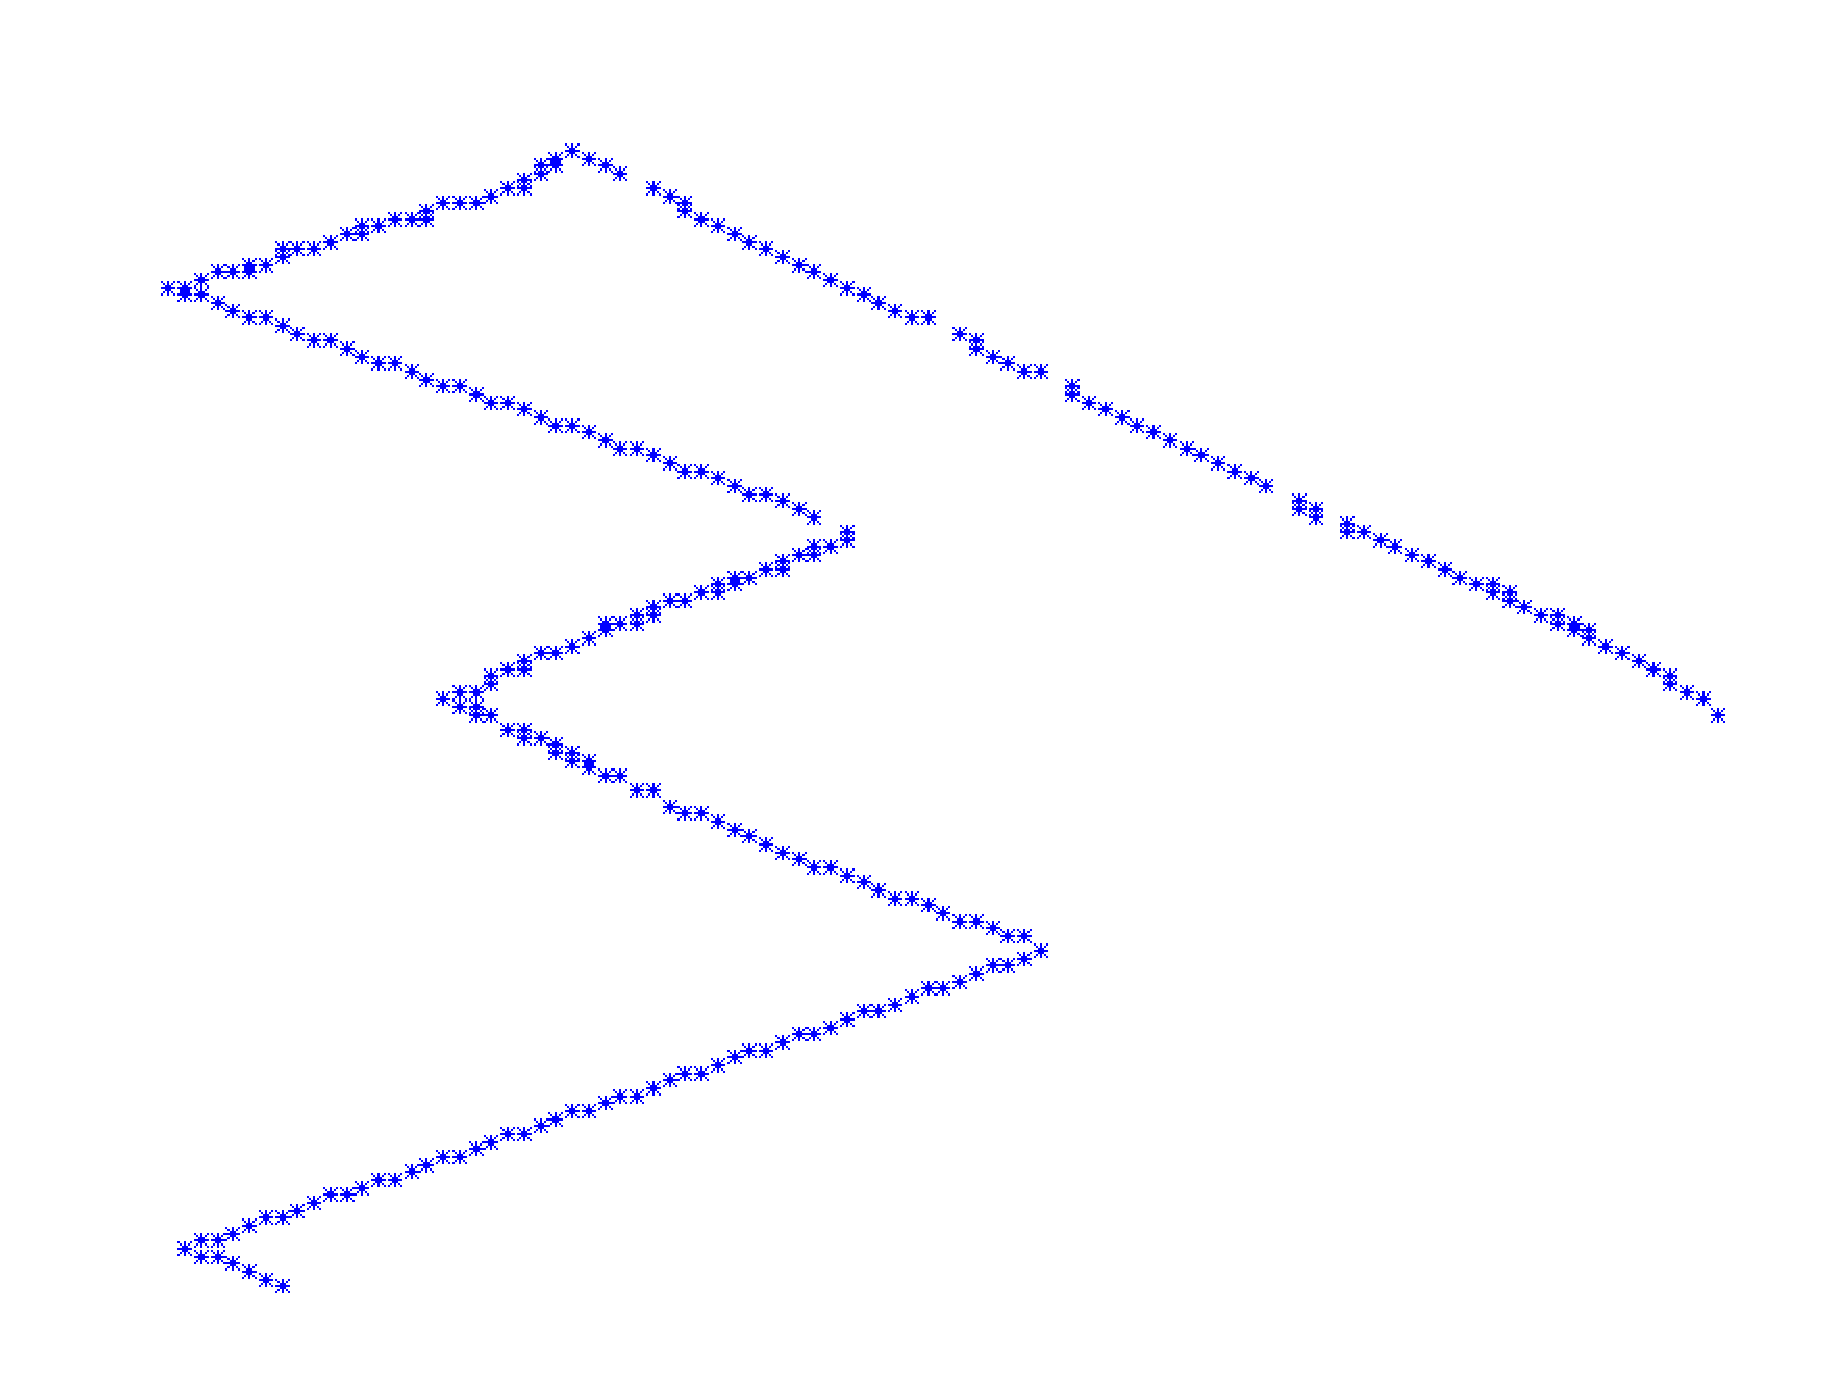
\includegraphics[width=0.4\textwidth,keepaspectratio]{images/get_line_example}
  \caption{Example of produced contour.}
	 \label{fig:get_line_example}
\end{figure}
In this step (Algorithm \ref{alg:ffd_contour_stage} lines
\ref{mark:ffd_contour_start}--\ref{mark:ffd_contour_end}) we use the
angle-sorted laser readings. The output of the contour step is a contour which
is built from the sorted laser readings. The algorithm computes the line that
lies between each two adjacent points from the set. The line is computed by
calling the function \textsc{Get-Line}. In our implementation we use
\emph{Bresenham's line algorithm} \cite{bresenham2010algorithm}. Next, all
points that are represented by all the lines (including the points from the
laser readings set) are merged into a contour (Figure \ref{fig:get_line_example}).

% 	\begin{figure}[htbp]
% 	 \centering
% 	 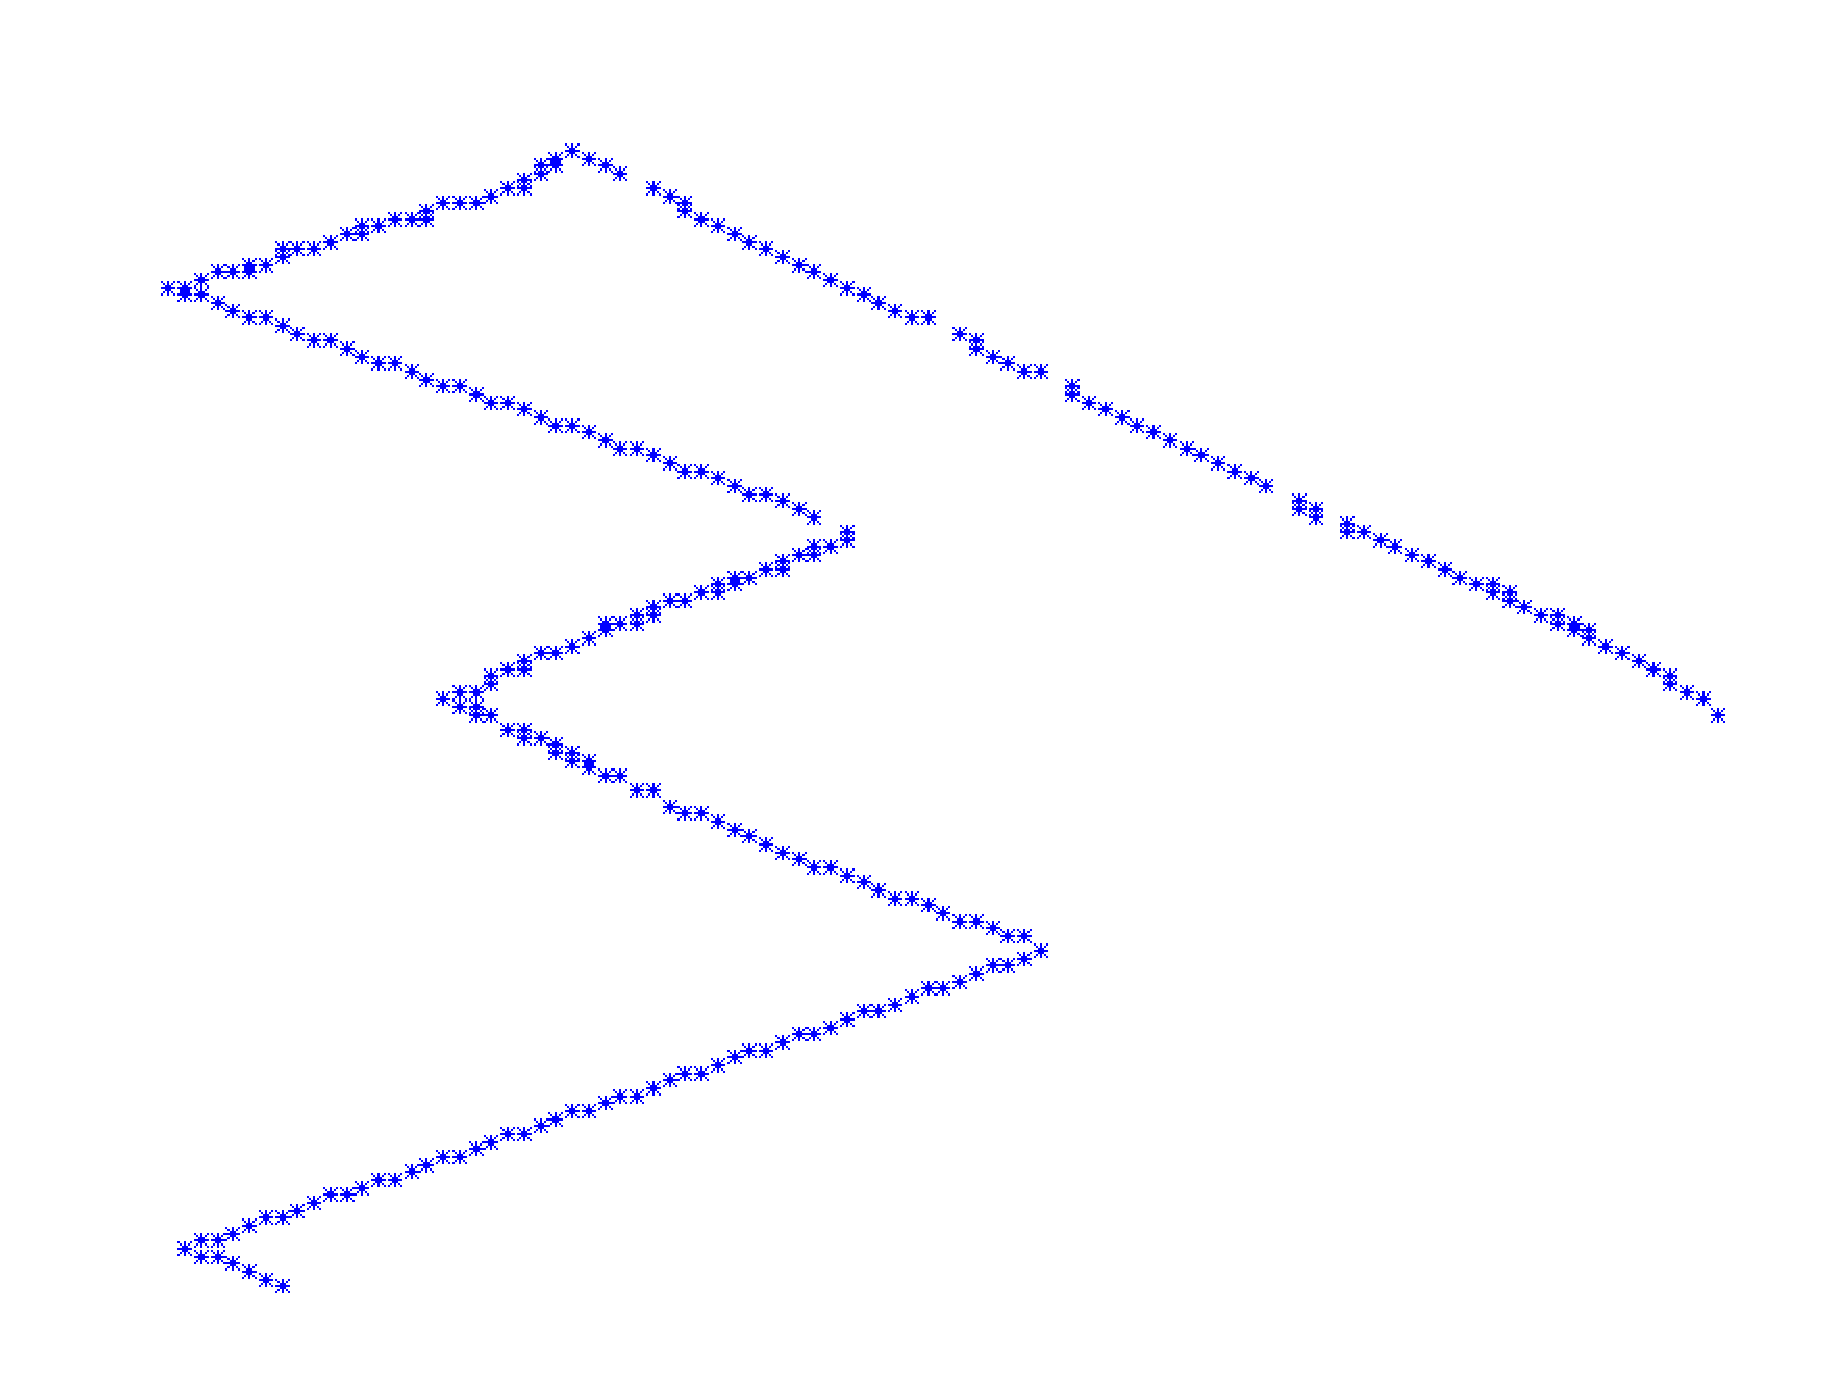
\includegraphics[width=0.4\columnwidth,keepaspectratio]{images/get_line_example}
% 	 \caption{Example of produced contour.} 	
% 	 \vspace{-15pt}
% 	 \label{fig:get_line_example}
% 	\end{figure}	



\begin{algorithm}[htbp]
\caption{Fast Frontier Detector (FFD): Extract Frontier Stage}
\label{alg:ffd_detect_new_frontier_stage}
\begin{algorithmic}[1]

\Require $contour$ 
\Comment{the contour built from the sorted laser readings}
\Ensure $NewFrontiers$
\Comment{list of new detected frontiers that lie on the contour}

\Function{Extract-Frontiers-1D}{$contour$}
\State{$NewFrontiers \gets \emptyset$} \Comment {list of new extracted
frontiers}
\label{mark:ffd_extract_start}

\State{$prev \gets POP(contour)$}

\If{$prev$ is a frontier cell} \Comment{special case}
	\State{create a new frontier in $NewFrontiers$}
\EndIf
\label{mark:ffd_special_case_end}

\ForAll {Point $curr \in contour$}
	\If {$curr$ is not a frontier cell}
	\label{mark:ffd_contour_eliminate_non_frontier_points}
		\State{$prev \gets curr$}
	\ElsIf {$curr$ has been visited before}
		\label{mark:ffd_redection_avoidance_start} 
		\State{$prev \gets curr$}
		\label{mark:ffd_redection_avoidance_end}
	\ElsIf {$curr$ and $prev$ are frontier cells}
		\State{add $curr$ to last created frontier}
		\State{$prev \gets curr$}
	\Else 
		\State{create a new frontier in $NewFrontiers$}
		\State{add $curr$ to last created frontier}
		\State{$prev \gets curr$}
	\EndIf
\EndFor 

\State \Return $NewFrontiers$
\label{mark:ffd_extract_end}
\EndFunction
\end{algorithmic}
\end{algorithm}
	\subsection{Detecting New Frontiers} \label{section:detecting_new_frontiers}
	In this step (Algorithm \ref{alg:ffd_detect_new_frontier_stage} lines
	\ref{mark:ffd_extract_start}--\ref{mark:ffd_extract_end}) the algorithm extracts new frontiers from the previously calculated contour. There are three cases correspond to each two adjacent points in the
	contour: 
	\begin{enumerate}
	\item \textbf{Current scanned point is not a frontier cell:} therefore,
	it does not contribute any new information about frontiers and can be ignored.
	
	\item \textbf{Current and previous scanned points are frontier cells:}
	therefore, both points belong to the same frontier and current scanned point is
	added to last detected frontier.
	
	% \yellownote{should we talk about that frontiers are either equal or disjoint?}
	\item \textbf{Current point is a frontier cell but the previous is
	not:} a new starting point of a frontier was detected. Hence, the algorithm creates a
	new frontier and adds the new starting point to it.
	\end{enumerate}


\begin{algorithm}[htbp]
\caption{Fast Frontier Detector (FFD): Maintenance of Previously Detected
Frontiers}
\label{alg:ffd_maintenance_stage}
\begin{algorithmic}[1]

\Require $NewFrontiers$
\Comment{list of new detected frontiers}
\Require $frontiersDB$
\Comment{data-structure that contains last known frontiers}
\Require $activeArea$
\Comment{data-structure that contains all points that lie inside the active
area}

\Function{Maintain-Frontiers}{$NewFrontiers,frontiersDB,activeArea$}

\ForAll {Point $p \in ActiveArea$}
\Comment{eliminate previously detected frontiers}
\label{mark:ffd_maintenance_start}
\label{mark:ffd_eliminating_previous_frontiers_start}
	\If {$p$ is a frontier cell} \label{mark:ffd_check_eliminate_of_frontier_point}

		\State{}		
		\Comment{split the current frontier into two partial frontiers}
		\State{get the frontier $f \in frontiersDB$ which enables $p \in f$}
		\label{mark:ffd_split_frontier_start}	
		\State{$f_1 \gets f[1\ldots p]$}
		\label{mark:split_start}
		\State{$f_2 \gets f[(p+1)\ldots |f|]$}
		\label{mark:split_end}
		\State{remove $f$ from $frontiersDB$}
		\State{add $f1$ and $f2$ to $frontiersDB$}
		\label{mark:ffd_split_frontier_end}
	\EndIf
\EndFor
\label{mark:ffd_eliminating_previous_frontiers_end}


\ForAll {Frontier $f \in NewFrontiers$}
\Comment{store new detected frontiers}
\label{mark:ffd_storing_new_frontiers_start}
	\If {$f$ overlaps with an existing frontier $ExistFrontier$}
		\State{$merged \gets f \cup ExistFrontier$}
		\State{remove $ExistFrontier$ from $frontiersDB$}
		\State{add $merged$ to $frontiersDB$}
	\Else 
		\State{create a new index and add $f$ to $frontiersDB$}	
	\EndIf
\EndFor
\label{mark:ffd_storing_new_frontiers_end}
\label{mark:ffd_maintenance_end}
\EndFunction
\end{algorithmic}
\end{algorithm}
	 
	\subsection{Maintaining Previously Detected
	Frontiers}\label{section:ffd_maintaining_previously_detected_frontiers} \FFD
	gains its speed by processing the laser readings only, rather than entire regions of the map.
	However, if the robot navigates towards a specific frontier, other previously
	detected frontiers are no longer updated because they are not covered by
	the robot's sensors. Thus, scanning the new received laser readings enables
	\FFD to detect only \emph{new} frontiers in each execution. In this step
	(Algorithm \ref{alg:ffd_maintenance_stage} lines
	\ref{mark:ffd_maintenance_start}--\ref{mark:ffd_maintenance_end}), in order to
	get complete information about the frontiers, the algorithm performs
	maintenance over previously detected frontiers which are no longer covered in
	the range of the sensors. Only by joining together new detected frontiers and
	previously detected frontiers, we get the overall frontiers in current world
	state. This step has multiple goals: avoiding detection of new frontiers in
	an already scanned area (Section \ref{section:avoiding_redetection}),
	eliminating frontier points which are no longer belong to frontiers (Section
	\ref{section:frontier_elimination}) and joining correctly the new detected
	frontiers together with previously detected frontiers (Section
	\ref{section:storing_frontiers}).
		
	
% 	\FFD requires the previously detected frontiers to be robust against
% 	map orientation changes caused by loop-closures of the mapping algorithm.
% 	In a \emph{Particle Filter} based SLAM infrastructures, changes in active
% 	particles probably occur. Hence, because particles do not share maps,
% 	each particle runs its own instance of \emph{FFD}.
	
% 	\subsubsection{Kalman Filter}
% 	The situation is different in \emph{Extended Kalman-Filter} (EKF) based SLAM
% 	infrastructures. These infrastructures have one map that is updated.
% 	Hence, data can be stored within a map in EKF SLAM infrastructures because the
% 	information about changing map orientation is available (in contrast to
% 	particle-based systems in which every particle is independent from the other
% 	particles).
	
	%EKF implementation contains one map which is updated by
	%the mapping algorithm (rather than several maps in Particle-Filter based SLAM
	%implementation)

	\subsubsection{The \FFD Data-Structures}
	In order to perform the maintenance step within a very short time as possible,
	\FFD utilizes two data-structures which have a short access time.  These data structures
        must maintain memory of frontiers between calls. Thus \FFD has to have persistent memory,
        i.e., data structures that persist between calls. This is contrast to
        other approaches that can be executed in a certain time, and only then. 

	Another thing to note is that in particle filter based systems (our focus in
	this thesis), each particle represents a possible hypothesis of the world state
	(including the robot position of course). The ``best'' particle is chosen
	according to a likelihood measurement. \FFD requires the previously detected
	frontiers to be robust against map orientation changes caused by loop-closures
	of the mapping algorithm.
	Therefore, when a new laser reading is received, \emph{each} particle executes
	its own instance of \FFD algorithm on its own map, using its own data structures. More
	specifically, each particle performs maintenance with its own map because
	particles do not share maps.
	We describe the data structures for maintenance below.
	
The first, \emph{Grid of Frontier Indices}, is an extension
of the occupancy grid (though it can be implemented as a separate entity). In
addition to occupancy information, each grid cell contains \textit{a frontier
index}, pointing to a frontier to which the grid cell belongs, or NULL
otherwise. The pointer points to a record stored in the Frontier Database
(described below).
In our implementation, we used integer index values. After accessing a grid cell
(Algorithm \ref{alg:ffd_maintenance_stage} Line
\ref{mark:ffd_check_eliminate_of_frontier_point}), querying for its frontier
index is $O(1)$.
	
	
% 	This data structure is a simple table in
% 	size of the grid which represents the world. Each cell contains either NULL,
% 	which represents that the cell is not a frontier cell, or an integer value,
% 	which represents that the cell is a frontier cell and belongs to the frontier
% 	whose index is that integer value. Using this grid of frontier indices
% 	enables us to quickly query wether a specific point in the world has been
% 	already declared as a frontier point. In our implementation, we expanded each
% 	map cell to have an additional attribute for storing its frontier index or
% 	NULL. Therefore, we could reuse the world map as the grid of frontier
% 	indices. After accessing a map cell, quering its frontier index is $O(1)$.
	
	The second, \emph{Frontier Database}, maps frontier
	indices (pointers) to sets of points ($frontierDB$ requirement of Algorithm
	\ref{alg:ffd_outline} and Algorithm \ref{alg:ffd_maintenance_stage}).
	All detected frontiers are stored in this data-structure. We use it to map frontier index to the actual set that
	contains the points in world coordinates. In our implementation, we use the
	default C++ implementation of a map template, which is implemented as a
	self-balancing binary search tree.
	Therefore, assuming $n$ represents the number of frontiers stored in the
	database, searching for a frontier index takes $O(\log n)$, inserting a new
	frontier takes $O(\log n)$ and removing a frontier index takes $O(\log n)$,
	though a (hash) table lookup implementation can make this faster.
	% XXX Matan, am I wrong about the hash table lookup?

	\subsubsection{Avoiding Re-Detection of Same Frontier}
	\label{section:avoiding_redetection}
	\FFD detects new frontiers by processing laser readings only.
	Hence, \FFD might detect the same frontier again and classify it as a new
	frontier if the robot did not change its position during two following \FFD
	executions. Moreover, if the robot travels back to an already visited
	region, no new frontiers should be detected. \FFD has to distinguish between
	laser readings from  between time frames. Otherwise, \FFD might wrongly detect
	a new frontier which lies within an already scanned area.

	Therefore, we keep track of the number of sensor visits (sensor covers) of each map cell. The
	definition of a frontier point is now expanded: a frontier point is a point
	which represent an unknown region, has at least one open-space neighbor and has
	not been scanned before. Given a contour, the detection of new frontiers ignores
	points that have already been scanned by the laser sensors and treats them as
	non-frontier points (Algorithm \ref{alg:ffd_detect_new_frontier_stage} lines
	\ref{mark:ffd_redection_avoidance_start}--\ref{mark:ffd_redection_avoidance_end}).

	Figure \ref{fig:redetecting_examples} demonstrates the necessity of the above.
	Figure \ref{fig:redetecting_bad} shows frontiers extraction
	without tracking the number of visits. It can be seen that there are frontiers that lie inside
	an open space area. This is absolutely wrong because frontiers are supposed to
	be positioned on the boundaries between known and unknown regions. In
	contrast, Figure \ref{fig:redetecting_good} shows frontiers extraction with
	avoidance of re-detecting same frontiers. It can be seen that every frontier
	separates known and unknown regions.
	
	\begin{figure}
	 \centering
	 \subfigure[Incorrectly re-detected frontiers.] {
	 \includegraphics[width=0.47\columnwidth,keepaspectratio]{images/redetecting_bad_example.eps}
	 \label{fig:redetecting_bad}}
	 \subfigure[Correct detection.] {
	 \centering
	 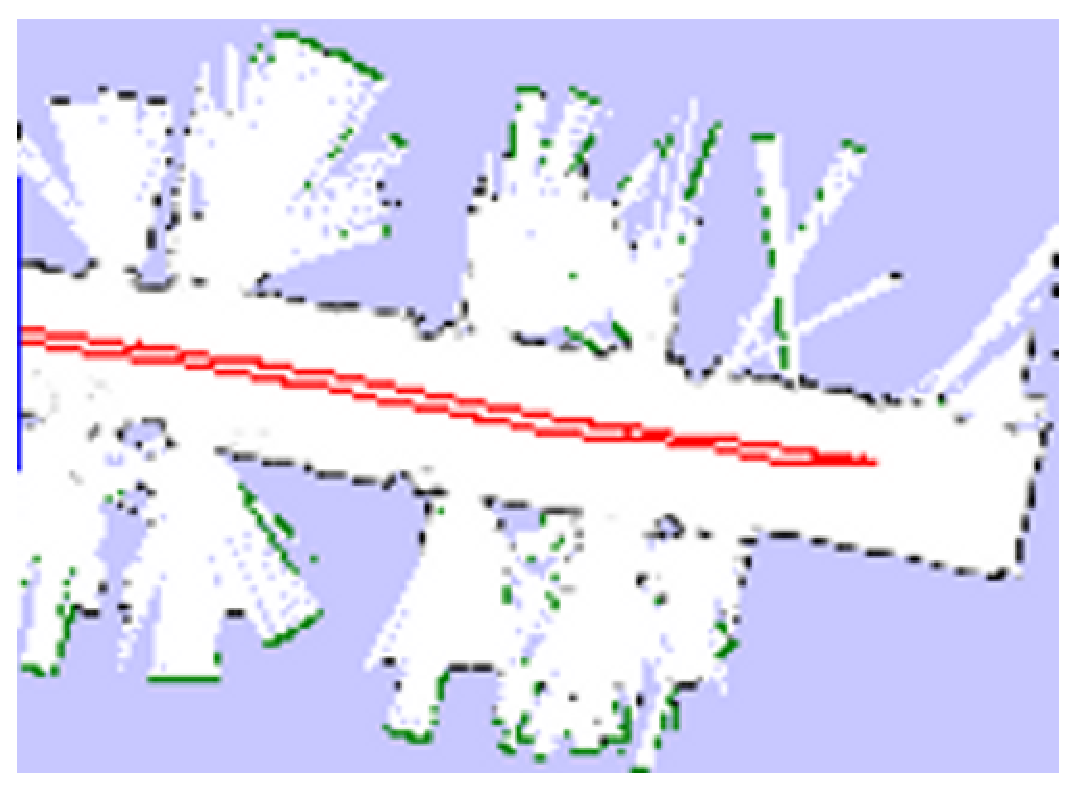
\includegraphics[width=0.47\columnwidth,keepaspectratio]{images/redetecting_good_example.eps}
	 \label{fig:redetecting_good}}
	 \caption{An example of re-detecting same frontiers.}
	 \label{fig:redetecting_examples}
	\end{figure}

	\subsubsection{Eliminating Previously Detected Frontiers}
	\label{section:frontier_elimination}
	In order to complete the process, points which are no longer in frontiers  (i.e. were
	covered by the robot's sensors) have to be eliminated. Lines
	\ref{mark:ffd_eliminating_previous_frontiers_start}--\ref{mark:ffd_eliminating_previous_frontiers_end}
	in Algorithm \ref{alg:ffd_maintenance_stage} contain the elimination logic
	applied by \FFD.

	%\paragraph{Active Area} 
	Let $t_i$ be a time frame and $lr_{t_i}$ be the laser readings which
	were received in time frame $t_i$. In order to perform maintenance in a specific
	time, we define the \emph{Active Area} of time frame $t_i$ to be the blocking
	rectangle that can be constructed using the farthest laser readings of
	$lr_{t_i}$, relative to the robot position in time frame $t_i$. 
	$$ x_{min} = min(\left\{x | x \in lr_{t_i} \right\}) ,
	 y_{min} = min(\left\{y | y \in lr_{t_i} \right\}) $$ 
	$$ x_{max} = max(\left\{x | x \in lr_{t_i} \right\}) ,
	 y_{max} = max(\left\{y | y \in lr_{t_i} \right\}) $$ 
	$$ActiveArea_{t_i} = \left\{\left(x,y \right) | x_{min}  \leq x \leq x_{max} ,
	y_{min}  \leq y \leq y_{max} \right\}$$ 
	The active area's rectangle is constructed from the following vertices: 
	$\left(x_{min},y_{min} \right)$,
	        $\left(x_{min},y_{max} \right)$,
	        $\left(x_{max},y_{max} \right)$,
	        $\left(x_{max},y_{min} \right)$. 
	The rectangle is an approximation to the real active area that is actually
	bounded within the laser readings. 
	%In the following section, we will explain
	%why the active area is a key feature in the process of maintaining frontiers.

% 	\subsubsection{Frontier Elimination}
	By processing received laser readings, \FFD extracts new frontiers.
	However, in order to get the complete world's frontiers state, points
	that are no longer on frontiers have to be eliminated. \FFD maintains a frontier
	database which maps an integer (frontier index) to a set of points (frontier).
	
	An unknown region is classified as known region only if it is covered by the
	robot's sensors. \FFD gets its input from the new received
	laser readings, and thus only regions that are covered by the
	robot's sensors might contain frontiers that have to be eliminated. Thus, if there are frontiers that need to be eliminated, they must
	lie inside the \emph{Active Area}. Hence, the active area is a key feature
	in the process of maintaining frontiers. \FFD scans each point that lies inside
	the active area and checks if it was previously belonged to a frontier. The
	check can be performed very fast as explained before. If the current scanned
	point was belonged to a frontier, the current scanned point is removed from
	the frontier and the frontier is splitted into two partial frontiers using the
	current scanned point as a pivot (Algorithm \ref{alg:ffd_maintenance_stage} lines
	\ref{mark:split_start}--\ref{mark:split_end}).
 
	In the end of this process, all no-longer frontier points in the frontier
	database are removed and the database contains only points that are still valid
	frontiers. 
	
	\subsubsection{Storing New Detected Frontiers}
	\label{section:storing_frontiers}	
	In the last phase of the maintenance step (Algorithm
	\ref{alg:ffd_maintenance_stage} lines
	\ref{mark:ffd_storing_new_frontiers_start}--\ref{mark:ffd_storing_new_frontiers_end})
	new detected frontiers are stored in the frontier database alongside with
	existing valid frontiers.  For each new detected frontier, \FFD checks if it
	overlaps with an already existing frontier. This comparison can be performed
	in a short time using the matrix of frontier indices. Each frontier point is
	queried in $O(1)$ operations. If an overlap is found, the frontier is merged
	with the frontier that it is overlapped with. If no overlap is found, then the
	frontier is inserted to the frontier database.
	
	
% 	We find \emph{Kalman-Filter} (EKF) based SLAM implementations best for
% 	integrating \FFD. In Section \ref{section:future_work}, we suggest a solution to
% 	integrate \FFD into Particle-Filter based SLAM implementations.
	
%\end{description}

% \input{algorithms/getContour} \input{algorithms/extractFrontiers}

% \yellownote{need to implement maintenance part of FFD}


\section{\FFD is Sound and Complete}
\label{section:ffd_sound_and_complete}
% \subsection{Completeness}
We show that Algorithm~\ref{alg:ffd_outline} is sound and complete.
We begin with a lemma that demonstrates that \FFD always recognizes new
frontiers (i.e., frontiers that appeared at time $t$, but did not exist before).
This will then be used to prove completeness of \FFD.
% \vspace{-7pt}
\begin{lemma}
\label{lem:newf}
Suppose $f$ is a frontier point at time $t$, which was not a frontier point at
any time $s$, where $s<t$. Then FFD will mark $f$ as a frontier given
observation $O_t$.
\end{lemma}
% \vspace{-10pt}
\begin{proof}
Let $f$ be a valid frontier point in time $t$ and was not classified as
frontier in time $s<t$. Since $f$ is a valid frontier point, then it has a
value of \emph{Unknown} and has at least one \emph{Open Space} neighbor at time
$t$. 
Assume towards a contradiction that \FFD did not recognize $f$ as a frontier
point. First, let us show that $f$ is contained in the contour handled
in Algorithm \ref{alg:ffd_detect_new_frontier_stage} lines
\ref{mark:ffd_extract_start}--\ref{mark:ffd_extract_end}.
Since $f$ is a valid frontier point, then it has a value
of \emph{Unknown} and has at least one \emph{Open Space} neighbor in time
$t$. The point $f$ cannot be located wholly within an \textit{unknown} region because it must
have at least one \emph{Open Space} neighbor. Also, the point $f$ cannot be
located wholly within a \textit{known} region since $f$ is a valid frontier point and
hence, its value is $Unknown$. Therefore, $f$ must be located on the contour
itself.
Lines \ref{mark:ffd_extract_start}--\ref{mark:ffd_extract_end} in Algorithm
\ref{alg:ffd_detect_new_frontier_stage} handle points on the contour, which we
have just shown $f$ is on. In these lines, the \FFD algorithm scans \emph{all}
contour points sequentially and specifically searches for frontier points.
Because it scans \emph{all} points on the contour, and we have shown that $f$
is on the contour, it follows that $f$ would be detected, contradicting the
assumption that \FFD did not recognize $f$ as a frontier point at time $t$.
\end{proof}
%\end{comment}

We now turn to proving the completeness of the \FFD algorithm. 
\begin{theorem}
 \label{thm:complete}
Let $f$ be a valid frontier point at time $t$. Then FFD will mark $f$ as a frontier point
given the sequence of observations $\langle O_0,\ldots,O_t\rangle$.
\end{theorem}

\begin{proof}
Two cases should be examined:

\noindent{\bf Case 1. $f$ is a new frontier point at time $t$.} Trivially,
this case is handled directly by lemma \ref{lem:newf}.

\noindent{\bf Case 2. $f$ was a new frontier point at time $s$, where $s<t$.}
Let $s$ be the earliest time in which $f$ was a frontier. Based on lemma 
\ref{lem:newf}, it follows that it was detected at this time. All that  remains
to show is that given $f$ is still valid at time $t$, \FFD will maintain
knowledge of it from time $s$ and report on it.
If $f$ is still a valid frontier point at time
$t$, then it has not been covered yet by the robot's sensors. Otherwise, it
would  no longer contain an \emph{Unknown} value and hence, would not
be a valid frontier point.  
So if it was not yet covered, it must be a frontier point that is maintained by 
\FFD. The only way in which $f$ can be eliminated from  being classified
as a frontier point is done by Algorithm \ref{alg:ffd_maintenance_stage} lines
\ref{mark:ffd_eliminating_previous_frontiers_start}--\ref{mark:ffd_eliminating_previous_frontiers_end}.
In these lines, \FFD scans all points that are covered by the robot's sensors
and checks if any points should be eliminated (Algorithm
\ref{alg:ffd_maintenance_stage} line
\ref{mark:ffd_check_eliminate_of_frontier_point}). Since $f$ is not covered by
the sensors, then it will not be scanned and eliminated in time $t$
$\Rightarrow$ $f$ remains classified as a frontier by \FFD.


In both cases we show \FFD will recognize $f$ to be a valid frontier at time $t$.
Since Theorem \ref{thm:complete} is true for any frontier point valid at time $t$,
it follows that \FFD is complete.   
\end{proof}
%\end{comment}


% \subsection{Soundness}
To show the soundness of \FFD, we must demonstrate that there does not exist a case
where \FFD marks a point $\hat{f}$ as a frontier, when it is not.

\begin{theorem}
\label{thm:sound}
Let $\hat{f}$ be an arbitrary point in the occupancy grid, which is \emph{not}
a frontier at time $t$. Then FFD will not return $\hat{f}$ as a frontier point,
given the sequence of observations $\langle O_0,\ldots,O_t\rangle$.
\end{theorem}

\begin{proof}
Assuming that $\hat{f}$ is an arbitrary point which is \emph{not} a frontier
point at time $t$, then $\hat{f}$ is either contains value different from
\emph{Unknown} or all its adjacent values are different from \emph{Open
Space}. We will examine two cases:

\noindent{\bf Case 1. $\hat{f}$ is marked as a new frontier.}
Suppose, towards a contradiction, that \FFD detects $\hat{f}$ as a new frontier
(i.e., true at time $t$, but not a frontier in time $s$, where $s<t$).
Since detection of new frontier points (Algorithm \ref{alg:ffd_detect_new_frontier_stage} lines
\ref{mark:ffd_extract_start}--\ref{mark:ffd_extract_end}) considers only points
on the contour, it follows that $\hat{f}$ must be located on the contour
\emph{and} detected by Algorithm \ref{alg:ffd_detect_new_frontier_stage} lines
\ref{mark:ffd_extract_start}--\ref{mark:ffd_extract_end}. However, Algorithm
\ref{alg:ffd_detect_new_frontier_stage} line \ref{mark:ffd_contour_eliminate_non_frontier_points}
specifically avoids classifying non-frontier points as frontiers. Since $\hat{f}$ is a non-frontier
point, it is ignored by \FFD. Therefore, $\hat{f}$ cannot be marked as a new
frontier $\Rightarrow$ contradicting the assumption that it is detected by \FFD
as a new frontier. Case 1 is impossible.

\noindent{\bf Case 2. $\hat{f}$ is an old frontier but was not
eliminated by the maintenance routine.} Suppose, towards a contradiction, that $\hat{f}$ is
located inside the active area and is not eliminated by the maintenance section.
Therefore, $\hat{f}$ is a point that was covered by the robot's sensors and no
longer contains an \emph{Unknown} value, yet is still marked as a frontier by
the \FFD algorithm.
We remind the the reader that in order to maintain frontier points across runs,
each point in the grid keeps a value which contains NULL if the point is not a
frontier point or the index of the frontier to whom it belongs.
Therefore, in Algorithm \ref{alg:ffd_maintenance_stage} line
\ref{mark:ffd_check_eliminate_of_frontier_point} \FFD scans all points in the
active area and checks if they contain a frontier index. When \FFD scans
$\hat{f}$, it finds out that it contains a valid frontier index (because it
has previously belonged to a valid frontier) and continues executing
Algorithm \ref{alg:ffd_maintenance_stage} lines
\ref{mark:ffd_split_frontier_start}--\ref{mark:ffd_split_frontier_end}. In
these lines, \FFD checks and removes from the frontier database all points that
are no longer frontier points and previously were frontier points. Thus,
$\hat{f}$ will be eliminated after scanning the active area, contradicting the
assumption that $\hat{f}$ was not eliminated.

Since in both cases we show that \FFD necessarily eliminated $\hat{f}$ from the
valid frontier list, it follows that if $\hat{f}$ is not a frontier-point at time $t$, it would not
be marked as such by \FFD.
Since Theorem \ref{thm:sound} holds for any arbitrary point, it follows that
\FFD never incorrectly marks a non-frontier point as a frontier. It is thus
sound.
\end{proof}
%\end{comment}



\section{Complexity Analysis}
\label{chap:complexity}
\section{Complexity}
\subsection*{WFD}

\begin{frame}
\frametitle{\WFD Complexity}
\begin{itemize}
  \item \WFD is based on Breadth-First Search (BFS) over the map.
  \item \WFD scans all \emph{Open Space} regions for frontier points.
  \item When a frontier point is found, another BFS is executed
  	\begin{itemize}
  	  \item in order to extract the frontier.
  	\end{itemize}
  \item BFS time complexity is linear in size of the search space.
  \item $\Rightarrow$ Linear in size of \emph{area} and \emph{perimeter} of
  \emph{Open Space} regions
\end{itemize}

$$
\order{\underbrace{S\term{open-space}}_{area} +
\underbrace{P\term{open-space}}_{perimeter}}
$$

\end{frame}

\begin{frame}
\frametitle{\WFD Best Case}
\begin{block}{Best Case}
The perimeter of the \openspace regions is minimal relatively to
the area of the \openspace regions
\end{block}
\begin{figure}
  \centering
  \def\bgColor{gray!15}

\def\createBackground{% The graphic
  \draw[fill=\bgColor] (-1.2,-1.2) -- (1.2,-1.2) -- (1.2,1.2) -- (-1.2,1.2) --
  (-1.2,-1.2);
 }


\definecolor{zubi}{RGB}{94,38,18}
\def\emphColor{zubi}
\def\arrowWidth{1pt}	
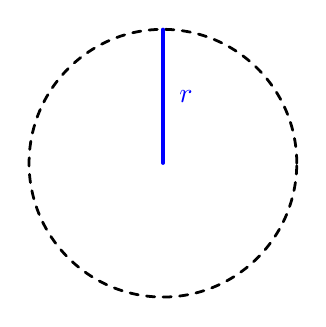
\begin{tikzpicture}[scale=\MyTikzScale,cap=round]
	  % Local definitions
	  \def\costhirty{0.8660256}
	  \def\cosforthyfive{0.7071067811}
	  % Colors
	  \colorlet{coscolor}{blue}
	
	  % Styles
	  \tikzstyle{axes}=[]
	  \tikzstyle{important line}=[very thick]
	  %\tikzstyle{information text}=[rounded corners,fill=red!10,inner sep=1ex]
	
	  % The graphic
	  %\draw[style=help lines,step=0.5cm] (-1.4,-1.4) grid (1.4,1.4);
	\createBackground 
	\draw[line width=1pt,dashed,fill=white] (0,0) circle (1cm);
	    
	   \draw[style=important line,coscolor]
	    (0,0) -- node[right=2pt,fill=none] {$r$}
	    (0,1);
	\end{tikzpicture}

	%\caption{\WFD Best Case: perimeter of \emph{open-space} regions is small as
	%possible}
	\label{fig:wfd_best_case}
\end{figure}
\end{frame}



\begin{frame}
\frametitle{\WFD Worst Case}
\begin{block}{Worst Case}
\begin{itemize}
  \item Maximize the length of the perimeter 
  	\begin{itemize}
  	  \item while \alert{keeping} the total area of the \openspace regions.
  	\end{itemize}
  \item Use a polygon as an approximation to a circle.
  \item The level of accuracy is determined by $k$, the number
of vertices.
\end{itemize}

\end{block}
\end{frame}



\begin{frame}
\frametitle{\WFD Worst Case}
\begin{figure}
\centering
\only<+>{\def\bgColor{gray!15}

\def\createBackground{% The graphic
  \draw[fill=\bgColor] (-1.2,-1.2) -- (1.2,-1.2) -- (1.2,1.2) -- (-1.2,1.2) --
  (-1.2,-1.2);
 }


\definecolor{zubi}{RGB}{94,38,18}
\def\emphColor{zubi}
\def\arrowWidth{1pt}
\begin{tikzpicture}[scale=\MyTikzScale,cap=round]
  % Local definitions
  \def\costhirty{0.8660256}
  \def\cosforthyfive{0.7071067811}
  % Colors
  \colorlet{coscolor}{blue}

  % Styles
  \tikzstyle{axes}=[]
  \tikzstyle{important line}=[very thick]
  %\tikzstyle{information text}=[rounded corners,fill=red!10,inner sep=1ex]

  \createBackground
    
%     \path (-0.2,-0.2) coordinate (A) (0.2,-0.2) coordinate (B)
%           (0.2,0.2) coordinate (C) (-0.2,0.2) coordinate (D);
%         \draw[fill=white] (A)--(B)--(C)--(D)--cycle;
        
    \newdimen \R
    \R=0.4cm
     \draw[fill=white] (45:\R) \foreach \x in {0,45,135,...,405} {
     	-- (\x:\R)
     } -- cycle (135:\R);

   \draw[style=important line,coscolor]
    (0,0) -- node[right=2pt,fill=none] {$r$}
    (90:\R);
    
    
    
    
    \foreach \x in {45,135,...,405} {
%  		\prev=67.5;
     	\path (\x:\R) coordinate (P1) ;
     	\path (45+\x:\R+0.7cm) coordinate (P2);
     	\path (90+\x:\R) coordinate (P3);
     	\draw[fill=white, dashed, line width=1pt] (P1) -- (P2) -- (P3);
    }
% 	\draw[fill=white] (22.5:\R) \foreach \x in {67.5,112.5,...,382.5} {
%      	-- (\x:\R)
%      }	
    
    %\draw[fill=white, line width=1pt,dashed] (A)--(0,-1.2)--(B);
    %\draw[fill=white] (B)--(BC)--(C)--cycle;
    %\draw[fill=white] (C)--(CD)--(D)--cycle;
    %\draw[fill=white] (D)--(DA)--(A)--cycle;

    \draw[style=important line,\emphColor]
    (-45:\R) -- node[left=0pt,fill=none] {}
    (45:\R);
    
    \draw[\emphColor]
    (\R-0.11cm,0) -- node[left=5pt,above=0pt,fill=none] {}
    (0.7cm+\R,0);
    
    \node[anchor=east] at (\R+\R,0) (src_h) {};
  	\node[color=\emphColor,anchor=west] at (45:1.3cm) (dst_h) {$h_{4}$};
  	\node[anchor=east] at (-30:0.866*\R) (src_b) {};
  	\node[color=\emphColor,anchor=west] at (-45:1.3cm) (dst_b) {$b_{4}$};
  	\draw[\emphColor,line width=\arrowWidth] (dst_h) edge[out=180,in=0,<->]
  	(src_h); 
  	\draw[\emphColor,line width=\arrowWidth] (dst_b) edge[out=180,in=0,<->]
  	(src_b);
  	
  	\node[anchor=east] at (\R*0.5,1.5*\R) (src_l) {};
  	\node[color=\emphColor,anchor=west] at (65.5:1.1cm) (dst_l) {$l_{4}$};
  	\draw[\emphColor,line width=\arrowWidth] (dst_l) edge[out=180,in=0,<->]
  	(src_l); \draw[fill=white, \emphColor,line width=2pt] (P1) -- (P2); %l4
  	
%     \draw[style=important line,red]
%     (0.3cm,0) -- node[left=5pt,above=0pt,fill=none] {$h_4$}
%     (2.6*\R,0);
    
\end{tikzpicture} \caption{$k=4$}}
\only<+>{\def\bgColor{gray!15}

\def\createBackground{% The graphic
  \draw[fill=\bgColor] (-1.2,-1.2) -- (1.2,-1.2) -- (1.2,1.2) -- (-1.2,1.2) --
  (-1.2,-1.2);
 }


\definecolor{zubi}{RGB}{94,38,18}
\def\emphColor{zubi}
\def\arrowWidth{1pt}
\begin{tikzpicture}[scale=\MyTikzScale,cap=round]
  % Local definitions
  \def\costhirty{0.8660256}
  \def\cosforthyfive{0.7071067811}
  % Colors
  \colorlet{coscolor}{blue}

  % Styles
  \tikzstyle{axes}=[]
  \tikzstyle{important line}=[very thick]
  %\tikzstyle{information text}=[rounded corners,fill=red!10,inner sep=1ex]

 	\createBackground   
    
    
    \newdimen \R
    \R=0.4cm
     \draw[fill=white] (22.5:\R) \foreach \x in {67.5,112.5,...,382.5} {
     	-- (\x:\R)
     } -- cycle (112.5:\R);

   \draw[style=important line,coscolor]
    (0,0) -- node[right=2pt,fill=none] {$r$}
    (0,0.37);
    
    
    \foreach \x in {22.5,67.5,112.5,...,381.5} {
%  		\prev=67.5;
     	\path (\x:\R) coordinate (P1);
     	\path (22.5+\x:\R+0.7cm) coordinate (P2);
     	\path (45+\x:\R) coordinate (P3);
     	\draw[fill=white, dashed, line width=1pt] (P1) -- (P2) -- (P3);
     	
     	%\draw (P3) -- (P1);
%      	\path (\x:\R) coordinate (x2\x)
    	%\path (0.5*\x+0.5*(\x+45):\R) coordinate (curr)
    	%\draw[fill=white] (prev) -- (curr)
    	%\draw[fill=white] (\x:\R) -- (\x:\R);
    	%\draw (0.5*(\prev+\x):\R) -- (\x:\R);
    }
    
% 	\draw[fill=white] (22.5:\R) \foreach \x in {67.5,112.5,...,382.5} {
%      	-- (\x:\R)
%      }	
    
    %\draw[fill=white, line width=1pt,dashed] (A)--(0,-1.2)--(B);
    %\draw[fill=white] (B)--(BC)--(C)--cycle;
    %\draw[fill=white] (C)--(CD)--(D)--cycle;
    %\draw[fill=white] (D)--(DA)--(A)--cycle;
\draw[style=important line,\emphColor]
    (-22.5:\R) -- node[left=0pt,fill=none] {}
    (22.5:\R);
    
%     \draw[style=important line,red]
%     (0:\R+0.1) -- node[left=10pt,above=1pt,fill=none] {$h_8$}
%     (\R+0.60cm,0);
    
    \draw[\emphColor]
    (\R-0.03cm,0) -- node[left=5pt,above=-5pt,fill=none] {}
    (0.7cm+\R,0);

	\node[anchor=east] at (\R+\R,0) (src_h) {};
  	\node[color=\emphColor,anchor=west] at (45:1.3cm) (dst_h) {$h_{8}$};
  	\node[anchor=east] at (-10:\R) (src_b) {};
  	\node[color=\emphColor,anchor=west] at (-45:1.3cm) (dst_b) {$b_{8}$};
  	\draw[\emphColor,line width=\arrowWidth] (dst_h) edge[out=180,in=0,<->]
  	(src_h); 
  	\draw[\emphColor,line width=\arrowWidth] (dst_b)
  	edge[out=180,in=0,<->] (src_b);
    
    \node[anchor=east] at (\R*0.35,1.5*\R) (src_l) {};
  	\node[color=\emphColor,anchor=west] at (67.5:1.1cm) (dst_l) {$l_{8}$};
  	\draw[\emphColor,line width=\arrowWidth] (dst_l) edge[out=180,in=0,<->]
  	(src_l); 
  	\draw[fill=white, \emphColor,line width=\arrowWidth] (67.5:\R) -- (90:\R+0.7cm); %l8
    
\end{tikzpicture}
 \caption{$k=8$}}
\only<+>{\def\bgColor{gray!15}

\def\createBackground{% The graphic
  \draw[fill=\bgColor] (-1.2,-1.2) -- (1.2,-1.2) -- (1.2,1.2) -- (-1.2,1.2) --
  (-1.2,-1.2);
 }


\definecolor{zubi}{RGB}{94,38,18}
\def\emphColor{zubi}
\def\arrowWidth{1pt}
\begin{tikzpicture}[scale=\MyTikzScale,cap=round]
  % Local definitions
  \def\costhirty{0.8660256}
  \def\cosforthyfive{0.7071067811}
  % Colors
  \colorlet{coscolor}{blue}

  % Styles
  \tikzstyle{axes}=[]
  \tikzstyle{important line}=[very thick]
  %\tikzstyle{information text}=[rounded corners,fill=red!10,inner sep=1ex]

	\createBackground    
%     \path (-0.2,-0.2) coordinate (A) (0.2,-0.2) coordinate (B)
%           (0.2,0.2) coordinate (C) (-0.2,0.2) coordinate (D);
%         \draw[fill=white] (A)--(B)--(C)--(D)--cycle;
    
    % top triangle
    \path (0,-1.2) coordinate (ABC) (1.2,0) coordinate (BC)
          (0,1.2) coordinate (CD) (-1.2,0) coordinate (DA);
    
    \newdimen \R
    \R=0.4cm
     \draw[fill=white] (11.25:\R) \foreach \x in {33.75,56.25,...,371.25} {
     	-- (\x:\R)
     } -- cycle (101.25:\R);

   \draw[style=important line,coscolor]
    (0,0) -- node[right=2pt,fill=none] {$r$}
    (90:\R);
    
    
    \foreach \x in {33.75,56.25,...,371.25}{%{22.5,67.5,112.5,...,381.5} {
%  		\prev=67.5;
     	\path (\x:\R) coordinate (P1);
     	\path (11.25+\x:\R+0.7cm) coordinate (P2);
     	\path (22.5+\x:\R) coordinate (P3);
     	\draw[fill=white, dashed, line width=1pt] (P1) -- (P2) -- (P3);
     	
     	%\draw (P3) -- (P1);
%      	\path (\x:\R) coordinate (x2\x)
    	%\path (0.5*\x+0.5*(\x+45):\R) coordinate (curr)
    	%\draw[fill=white] (prev) -- (curr)
    	%\draw[fill=white] (\x:\R) -- (\x:\R);
    	%\draw (0.5*(\prev+\x):\R) -- (\x:\R);
    }
    
% 	\draw[fill=white] (22.5:\R) \foreach \x in {67.5,112.5,...,382.5} {
%      	-- (\x:\R)
%      }	
    
    %\draw[fill=white, line width=1pt,dashed] (A)--(0,-1.2)--(B);
    %\draw[fill=white] (B)--(BC)--(C)--cycle;
    %\draw[fill=white] (C)--(CD)--(D)--cycle;
    %\draw[fill=white] (D)--(DA)--(A)--cycle;
\draw[style=important line,\emphColor]
    (-11.25:\R) -- node[left=0pt,fill=none] {}
    (11.25:\R);
    
%     \draw[style=important line,red]
%     (0:\R+0.1) -- node[left=10pt,above=1pt,fill=none] {$h_8$}
%     (\R+0.60cm,0);
    
    \draw[\emphColor]
    (\R-0.01cm,0) -- node[left=5pt,above=-5pt,fill=none] {}
    (0.7cm+\R,0);
    
    \node[anchor=east] at (\R+\R,0) (src_h) {};
  	\node[color=\emphColor,anchor=west] at (45:1.3cm) (dst_h) {$h_{16}$};
  	\node[anchor=east] at (-5:\R) (src_b) {};
  	\node[color=\emphColor,anchor=west] at (-45:1.3cm) (dst_b) {$b_{16}$};
  	\draw[\emphColor,line width=\arrowWidth] (dst_h) edge[out=180,in=0,<->]
  	(src_h); 
  	\draw[\emphColor,line width=\arrowWidth] (dst_b) edge[out=180,in=0,<->]
  	(src_b);
    
    \node[anchor=east] at (\R*0.20,1.5*\R) (src_l) {};
  	\node[color=\emphColor,anchor=west] at (80:1.1cm) (dst_l) {$l_{16}$};
  	\draw[\emphColor,line width=\arrowWidth] (dst_l) edge[out=180,in=0,<->]
  	(src_l); \draw[fill=white, \emphColor,line width=2pt] (78.75:\R) -- (90:\R+0.7cm); %l8
    
\end{tikzpicture}
 \caption{$k=16$}}
\only<+>{\def\bgColor{gray!15}

\def\createBackground{% The graphic
  \draw[fill=\bgColor] (-1.2,-1.2) -- (1.2,-1.2) -- (1.2,1.2) -- (-1.2,1.2) --
  (-1.2,-1.2);
 }


\definecolor{zubi}{RGB}{94,38,18}
\def\emphColor{zubi}
\def\arrowWidth{1pt}
\begin{tikzpicture}[scale=\MyTikzScale,cap=round]
  % Local definitions
  \def\costhirty{0.8660256}
  \def\cosforthyfive{0.7071067811}
  % Colors
  \colorlet{coscolor}{blue}

  % Styles
  \tikzstyle{axes}=[]
  \tikzstyle{important line}=[very thick]
  %\tikzstyle{information text}=[rounded corners,fill=red!10,inner sep=1ex]

  % The graphic
  \createBackground   
    
%     \path (-0.2,-0.2) coordinate (A) (0.2,-0.2) coordinate (B)
%           (0.2,0.2) coordinate (C) (-0.2,0.2) coordinate (D);
%         \draw[fill=white] (A)--(B)--(C)--(D)--cycle;
        
    \newdimen \R
    \R=0.4cm
    
     \draw[fill=white] (5.625:\R) \foreach \x in {16.875,22.56,...,365.62} {
     	-- (\x:\R)
     } -- cycle (95.625:\R);

   \draw[style=important line,coscolor]
    (0,0) -- node[right=2pt,fill=none] {$r$}
    (90:\R);
    
    
    \foreach \x in {5.625,11.25,...,365.62} {
%  		\prev=67.5;
     	\path (\x:\R) coordinate (P1);
     	\path (5.625+\x:\R+0.7cm) coordinate (P2);
     	\path (11.25+\x:\R) coordinate (P3);
     	\draw[fill=white, dashed, line width=1pt] (P1) -- (P2) -- (P3);
     	
     	%\draw (P3) -- (P1);
%      	\path (\x:\R) coordinate (x2\x)
    	%\path (0.5*\x+0.5*(\x+45):\R) coordinate (curr)
    	%\draw[fill=white] (prev) -- (curr)
    	%\draw[fill=white] (\x:\R) -- (\x:\R);
    	%\draw (0.5*(\prev+\x):\R) -- (\x:\R);
    }
    
% 	\draw[fill=white] (22.5:\R) \foreach \x in {67.5,112.5,...,382.5} {
%      	-- (\x:\R)
%      }	
    
    %\draw[fill=white, line width=1pt,dashed] (A)--(0,-1.2)--(B);
    %\draw[fill=white] (B)--(BC)--(C)--cycle;
    %\draw[fill=white] (C)--(CD)--(D)--cycle;
    %\draw[fill=white] (D)--(DA)--(A)--cycle;
\draw[style=important line,\emphColor]
    (-5.625:\R) -- node[left=0pt,fill=none] {$b_{32}$}
    (5.625:\R);
    
%     \draw[style=important line,red]
%     (0:\R+0.1) -- node[left=10pt,above=1pt,fill=none] {$h_8$}
%     (\R+0.60cm,0);
    
    \draw[\emphColor]
    (\R,0) -- node[left=5pt,above=-5pt,fill=none] {}
    (0:0.7cm+\R);
%     (\R-0.01cm,0) -- node[left=5pt,above=-5pt,fill=none] {$h_{32}$}
%     (0.7cm+\R,0);

  	\node[anchor=east] at (\R+\R,0) (src_h){};
  	\node[color=\emphColor,anchor=west] at (45:1.3cm) (dst_h) {$h_{32}$};
  	\node[anchor=east] at (\R,0) (src_b) {};
  	\node[color=\emphColor,anchor=west] at (-45:1.3cm) (dst_b) {$b_{32}$};
  	\draw[\emphColor,line width=\arrowWidth] (dst_h) edge[out=180,in=0,<->]
  	(src_h); \draw[\emphColor, line width=\arrowWidth] (dst_b)
  	edge[out=180,in=0,<->] (src_b);

    \node[anchor=east] at (\R*0.65,1.5*\R) (src_l) {};
  	\node[color=\emphColor,anchor=west] at (60:1.3cm) (dst_l) {$l_{32}$};
  	\draw[\emphColor,line width=\arrowWidth] (dst_l) edge[out=180,in=0,<->]
  	(src_l); 
  	\draw[fill=white, \emphColor,line width=2pt] (67.5:\R) -- (71.125:\R+0.7cm);
  	%l8
    
\end{tikzpicture} \caption{$k=32$}}
\end{figure}
\end{frame}

\begin{frame}
\label{frame:wfd_complexity}
\frametitle{\WFD Worst Case}
Run-time complexity of \WFD in terms of \openspace area: 
$$
  \order{S_{open}\cdot 
  \term{
  1+
  \sqrt{\term{\frac{1}{r\cdot\tan{\frac{\pi}{S_{open}}}}}^2
        -\frac{1}{\tan{\frac{\pi}{S_{open}}}} + r^2}}}
  $$  
\hyperlink{frame:wfd_complexity_details}{\beamergotobutton{Complexity in
Details}}
\end{frame}


\subsection*{FFD}
\begin{frame}
\frametitle{\FFD Complexity}
\begin{itemize}
  \item It may seem that \FFD's complexity is contained within \WFD
  	\begin{itemize}
  	  \item since \FFD searches only inside the active area (\openspace)
  	\end{itemize}
  \item It is not true since \FFD has to persistently run in the background
  \item We analyse the complexity of each stage separatly
\end{itemize}
\end{frame}


\begin{frame}
\label{frame:ffd_complexity}
\frametitle{\FFD Complexity}
\begin{itemize}
  \item $\execTime{c}:=$ the length of the contour in time $t$
  \item $\execTime{n_f}:=$ number of frontiers in the frontier database in time
  $t$
  \item Single execution:
   $$\order{\execTime{c} +
        \log{\execTime{n_f}}}  
   $$
  \item \FFD has to run in the background  
  \begin{itemize}
    \item $l_\omega:=$ frequency of the laser sensor
    \item $t_{m}:=$ worst-case elapsed time between two following map-events
    \item $P_n:=$ number of particles in the SLAM implementation
    $$
    \order{P_n\cdot \term{t_m \cdot l_\omega} \cdot\term{\execTime{c} +
        \log{\execTime{n_f}}}} 
    $$
  \end{itemize}
\end{itemize}
\hyperlink{frame:ffd_complexity_details}{\beamergotobutton{Complexity in
Details}}
\end{frame}

\section{About Maintenance and Improving \WFD}
\label{chap:maint}
The \WFD algorithm does not separate old and new frontiers and 
therefore, has to detect them with each execution. Therefore, \WFD's search
domain is bounded to the whole map. In contrast, \FFD algorithm is able to detect new frontiers
only. In order to enable \FFD eliminating previously detected frontiers, it has
to persistently perform a maintenance. 
%The general maintenance algorithm is
%shown in Algorithm \ref{alg:wfd_maintenance}. This algorithm is quite similar
%the \FFD's maintenance algorithm (Algorithm \ref{alg:ffd_maintenance_stage})
% but with a slight modification (active area as input argument). 
The general maintenance algorithm is shown in Section \ref{chap:ffd} (Algorithm
\ref{alg:ffd_maintenance_stage}). In this
section we discuss the general concepts of the maintenance process
(Section \ref{section:general_maintenenace_concepts}) and present two
algorithms which represent a hybrid version of both \WFD and \FFD (the
former is discussed in Section \ref{section:wfd_incremental} and the
latter is discussed in Section \ref{section:wfd_incremental_parallel}).

\subsection{General Maintenance Concepts}
\label{section:general_maintenenace_concepts}

In Section \ref{section:ffd_maintaining_previously_detected_frontiers}, we
showed and explained the maintenance stage of the \FFD algorithm (Algorithm
\ref{alg:ffd_maintenance_stage}). This process can be generalized
and applied to other frontier detection algorithms. By applying maintenance, we
can separate between the two parts that any frontier detection needs to handle:
detection of new frontiers and elimination of existing frontiers. 

The presented maintenance algorithm (Algorithm \ref{alg:ffd_maintenance_stage})
is not bounded to a specific frontier detection algorithm. The algorithm gets
its inputs and acts independently. We encourage the reader
to find more details in Section
\ref{section:ffd_maintaining_previously_detected_frontiers}.
By integrating the maintenance algorithm into \WFD, the frontier search domain
can now be reduced (similar to \FFD). 
%\begin{algorithm}[htbp]
\caption{Generic Frontier Maintenance}
\label{alg:wfd_maintenance}
\begin{algorithmic}[1]

\Require $NewFrontiers$
\Comment{list of new detected frontiers}
\Require $frontiersDB$
\Comment{data-structure that contains last known frontiers}
\Require $activeArea$
\Comment{data-structure that contains all points that lie inside the active
area}

\Function{Maintenance}{$activeArea$,$NewFrontiers,frontiersDB$}

\ForAll {Point $p \in ActiveArea$}
\Comment{eliminate previously detected frontiers}
	\If {$p$ is a frontier cell} 

		\State{}		
		\Comment{split the current frontier into two partial frontiers}
		\State{get the frontier $f \in frontiersDB$ which enables $p \in f$}
		
		\State{$f_1 \gets f[1\ldots p]$}
		\State{$f_2 \gets f[(p+1)\ldots |f|]$}
		\State{remove $f$ from $frontiersDB$}
		\State{add $f1$ and $f2$ to $frontiersDB$}
	\EndIf
\EndFor



\ForAll {Frontier $f \in NewFrontiers$}
\Comment{store new detected frontiers}

	\If {$f$ overlaps with an existing frontier $existFrontier$}
		\State{$merged \gets f \cup existFrontier$}
		\State{remove $existFrontier$ from $frontiersDB$}
		\State{add $merged$ to $frontiersDB$}
	\Else 
		\State{create a new index and add $f$ to $frontiersDB$}	
	\EndIf
\EndFor

\EndFunction
\end{algorithmic}
\end{algorithm}


For instance, we integrated the maintenance mechanism into \WFD
algorithm and created two advanced versions of it which are presented in the
following sections. The first, an incremental version of \WFD is called
\WFDINC, and the second, a parallel version which is called \WFDIP.

\subsection{Incremental Wavefront Frontier Detector}
\label{section:wfd_incremental}
Our first \WFD improvement is called \WFDINC (Algorithm
\ref{alg:WavefrontFrontierDetectorIncremental}). In this version of \WFD,
instead of searching the whole map for frontier points, the search domain
contains only points that lie inside the active area. The idea is based on
the proof in Section \ref{section:ffd_sound_and_complete}; the only region in
the map that contains changes (i.e. contains new frontiers and contains
frontiers that are needed to be eliminated) is the active area. We define the
active area to be the bounding rectangle that is constructed using the farthest
laser readings received from last executions of \WFDINC.

\begin{singlespace}
\begin{algorithm}[htbp]
\caption{Incremental Wavefront Frontier Detector (WFD-INC)}
\label{alg:WavefrontFrontierDetectorIncremental}
\begin{algorithmic}[1]

\Require{$queue_m$} \Comment{queue, used for detecting frontier
points from a given map} 
 
\Require{$pose$} \Comment{current global position of the
robot}

\Require \colorbox{Gray}{$frontiersDB$}
\Comment{data-structure that contains last known frontiers}

%%%%%%%%%%%%%%%%%%%%%%%%%%%%%%%%%%%%%%%%%%%%%%%%%%%%%%%%%%%%%%%
\Function{WFD-INC}{$activeArea,Map,pose, frontiersDB$}

\If {\colorbox{Gray}{best particle index was changed from last execution}}
\label{mark:wfdinc_particle_changed_start}
	\State {\colorbox{Gray}{clear all data from $frontiersDB$}}
	\State {\colorbox{Gray}{$activeArea \gets Map$ }} \Comment{active
	area contains all map points}
\EndIf
\label{mark:wfdinc_particle_changed_end}

\State{$queue_m \gets \emptyset$}
\State{$newFrontiers \gets \emptyset$}

\State {\Call {Enqueue}{$queue_m$, $pose$}}

\State {mark $pose$ as ``Map-Open-List''} 
\Statex{}
\While {$queue_m$ is not empty}

	\State{$p \gets$ \Call {Dequeue}{$queue_m$}}
	 
	\If{$p$ is marked as ``Map-Close-List''}
		\State{continue}
	\EndIf 
	
	\If{$p$ is a frontier point}
		\State{$foundFrontier \gets$ \Call {Extract-Frontier-2D}{$p$}}
		\State{add $foundFrontier$ to $newFrontiers$}
		\State{mark all points of $foundFrontier$ as ``Map-Close-List''}
	\EndIf \newline
	
	\ForAll{$v \in adj(p)$}
		\If{$v$ not marked as \{``Map-Open-List'', ``Map-Close-List''\} 
		 \textbf{and} $v$ has at least one ``Map-Open-Space'' neighbor 
		 \colorbox{Gray}{\textbf{and} $v \in activeArea$} }
		\label{mark:wfdinc_check_if_in_active_area}
		
			\State{\Call {Enqueue}{$queue_m$,$v$}}
		
			\State{mark $v$ as ``Map-Open-List''}
		\EndIf
	\EndFor \newline
	
	\State{mark $p$ as ``Map-Close-List''}
	%\State{\colorbox{Gray}{mark $p$ as ``visited''}}
\EndWhile


\State{\colorbox{Gray}{\Call {Maintain-Frontiers}{$newFrontiers,
frontiersDB,activeArea$}}}
\label{mark:wfdinc_call_maintenance}
\EndFunction
\end{algorithmic}
\end{algorithm}
\end{singlespace}

 
Similar to State-of-the-art frontier detection algorithms, \WFD
has to detect all frontiers in each execution. \WFD has better performance
than State-of-the-art frontier detection algorithm since it has a smaller search
domain. However, comparing to \FFD, it is still limited. If there were
not changes in map orientation, then all previous frontiers should keep their
map coordinates. 

The \WFDINC algorithm exploits this fact and scans only regions
that might contain changes in frontiers (i.e. regions which were hit by the
laser sensors). If a map orientation was changed (Lines
\ref{mark:wfdinc_particle_changed_start}--\ref{mark:wfdinc_particle_changed_end}),
then all previous frontier data is cleared and the
algorithm start detecting all frontiers in the same way as \WFD algorithm.
Another modification from original \WFD algorithm is when checking the adjacent
points of current scanned point (Line
\ref{mark:wfdinc_check_if_in_active_area}). In this version of \WFD, only points
that lie inside the active area are scanned. This reduces the size of the search
domain. The last modification from the original \WFD algorithm is that a
maintenance has to be called, since \WFDINC does not search over the whole map
(Line \ref{mark:wfdinc_call_maintenance}).     

Both \WFD (Algorithm \ref{alg:WavefrontFrontierDetector1}) and \WFDINC
(Algorithm \ref{alg:WavefrontFrontierDetectorIncremental}) share many common code lines.
We highlighted the differences between both algorithms in order to help the reader
to notice the differences between them more easily.
%



\subsection{Incremental-Parallel Wavefront Frontier Detector}
\label{section:wfd_incremental_parallel}
Our second improvement of \WFD is actually an improvement of \WFDINC and called
\WFDIP. If changes in map orientations happen too often, then \WFDINC's
performance is the same as \WFD (but now including an overhead of maintenance).
Our goal is therefore to artificially reduce the number of changes in map
orientation as much as possible. The solution is simple: \WFDIP keeps a separate
instance of \WFDINC algorithm for each particle. Whenever \WFDIP is executed, it executes
each instance of \WFDINC according to each particle's map data. Therefore, all
instances of \WFDINC never reach lines
\ref{mark:wfdinc_particle_changed_start}--\ref{mark:wfdinc_particle_changed_end}
and keep frontier data between executions is guaranteed. 
\begin{algorithm}[htbp]
\caption{Incremental-Parallel Wavefront Frontier Detector (WFD-IP)}
\label{alg:WavefrontFrontierDetectorIncrementalParallel}
\begin{algorithmic}[1]
\Require{$particles$} \Comment{data-structure that contains all particles of the
SLAM implemantation}
%%%%%%%%%%%%%%%%%%%%%%%%%%%%%%%%%%%%%%%%%%%%%%%%%%%%%%%%%%%%%%%
\ForAll{Particle $p \in particles$}
	\State{\Call{WFD-INC}{$p\to activeArea$, $p\to Map$, $p\to pose$,
	$p\to frontiersDB$}}
\EndFor
\end{algorithmic}
\end{algorithm}



\section{Experimental Results}
\label{chap:results}
\section{Experimental Results}

% \begin{frame}<beamer>
% \frametitle{Outline}
% \tableofcontents[currentsection,currentsubsection]
% \end{frame}
\subsection*{Experiment Design}
\begin{frame}
\frametitle{Experiment Design}
\begin{itemize}
  \item We have fully implemented \WFD, \WFDINC, \WFDIP and \FFD 
  \item We compare all algorithms with a State-of-the-Art algorithm\footnote{We
  thank Kai M. Wurm and Wolfram Burgard for providing us their own
  implementation}
  \item Our system is based on \emph{GMapping} SLAM implementation
  	\begin{itemize}
  		\item \citep{grisetti05icra,grisetti07tro} 
  	\end{itemize} 
  \item Two machines: 
  	\begin{itemize}
  		\item Intel Core 2 Duo T6600 CPU, 2.20GHz, 4GB RAM
  		\item Intel Pentium III Coppermine CPU, 800MHz, 1GB RAM % not going to talk
  		% d about former results
  	\end{itemize} 
  \item We measured CPU-process time 
\end{itemize}
\end{frame}

\begin{frame}
\frametitle{Experiment Design}
\begin{itemize}
  \item All detection algorithms are executed when a map update occurs 
  \item \FFD is executed when a new laser reading is received 
  \item We accumulate \FFD's time between two map updates
  %calls to other algorithms
  \item Tested on data obtained from RADISH \citep{Radish}
  	\begin{itemize}
  	  \item Gold standard robotics dataset
  	  \item Provides exploration data obtained by \emph{real-world} robots
  	  %\item Gold standard of exploration community
  	  \item Tested on all maps contain exploration range readings data  
  	\end{itemize}  
\end{itemize}
\end{frame}


% \begin{frame}
% \frametitle{Experiment Design}
% \transdissolve
% 	\begin{figure}
% 	 \centering
% 	 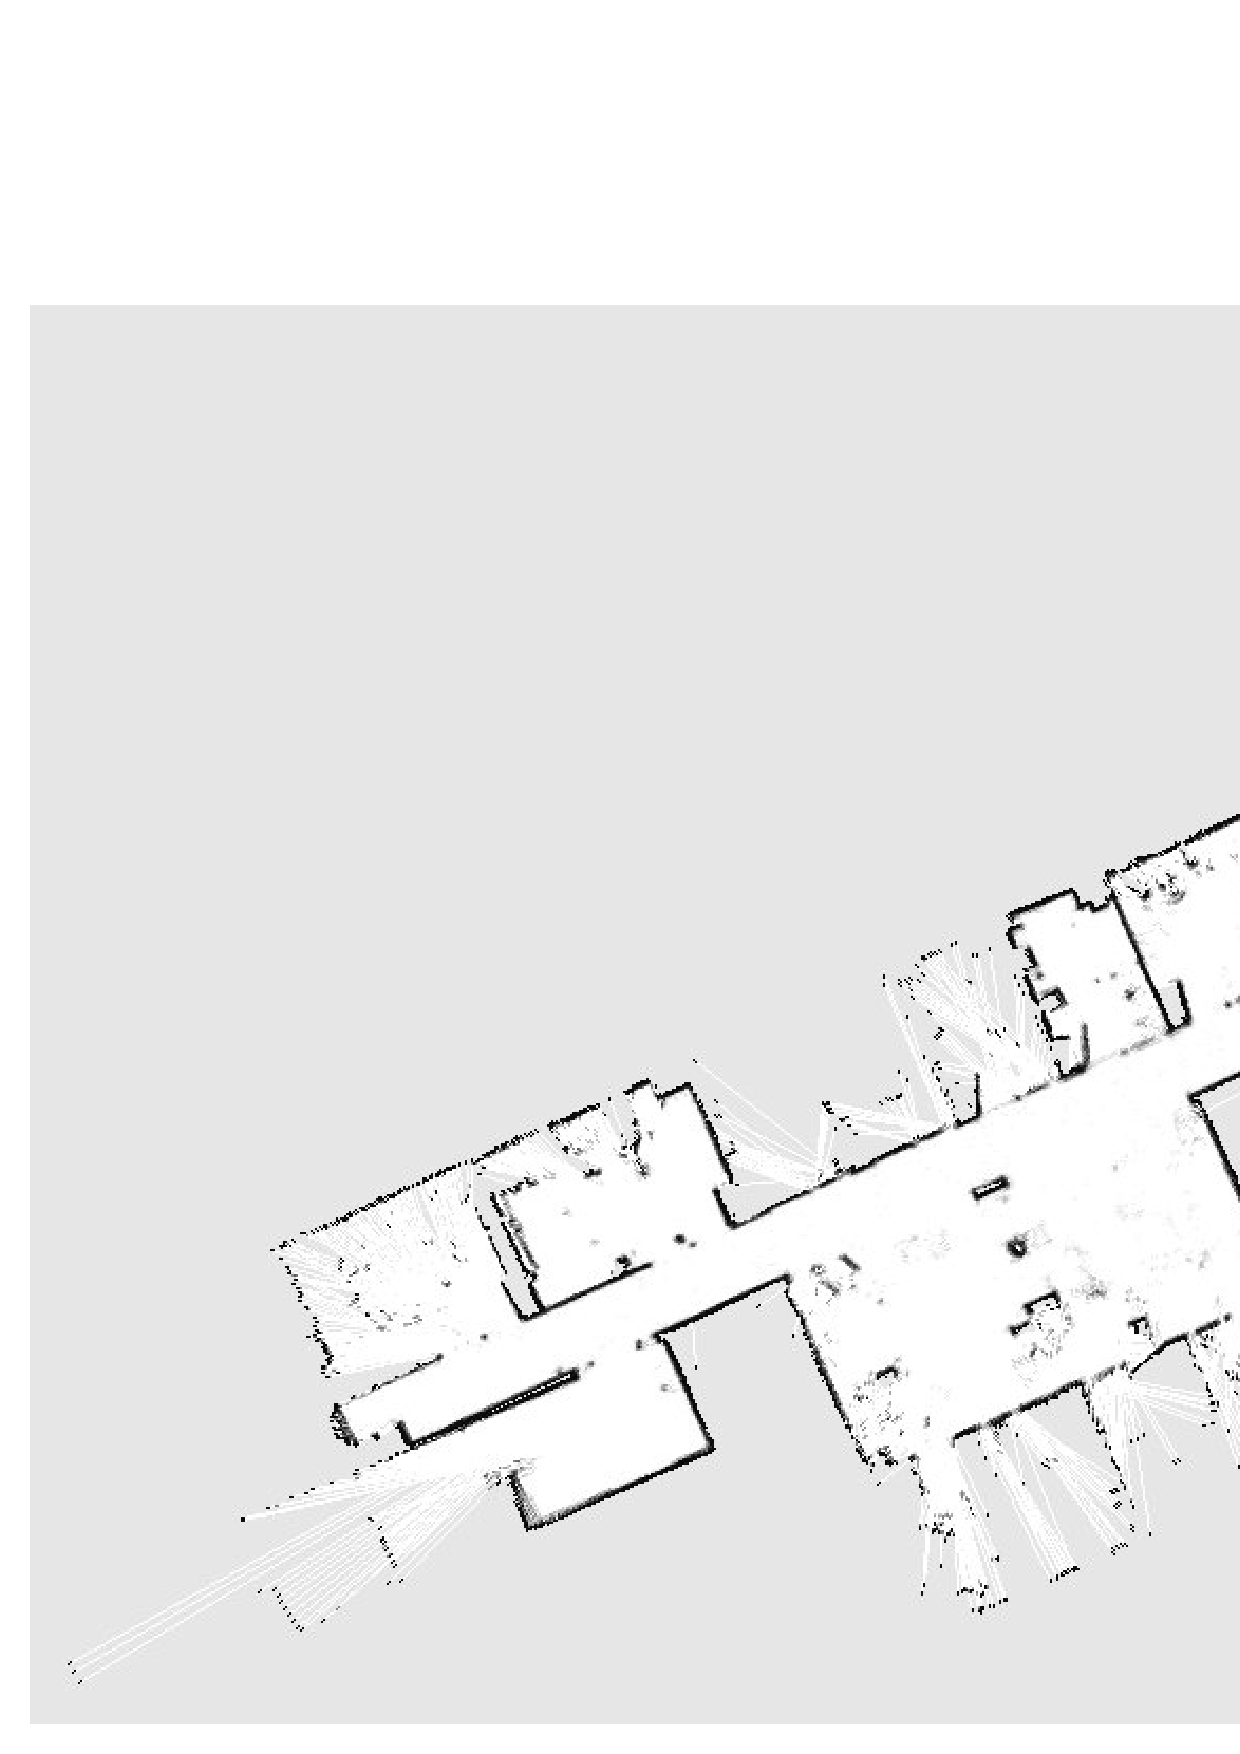
\includegraphics[width=0.85\columnwidth,keepaspectratio]{images/cartesium.JPG}
% 	\end{figure}
% \end{frame}


\begin{frame}
\frametitle{Experiment Design}
\transfade%\transdissolve
	\begin{figure}
	 \centering
	 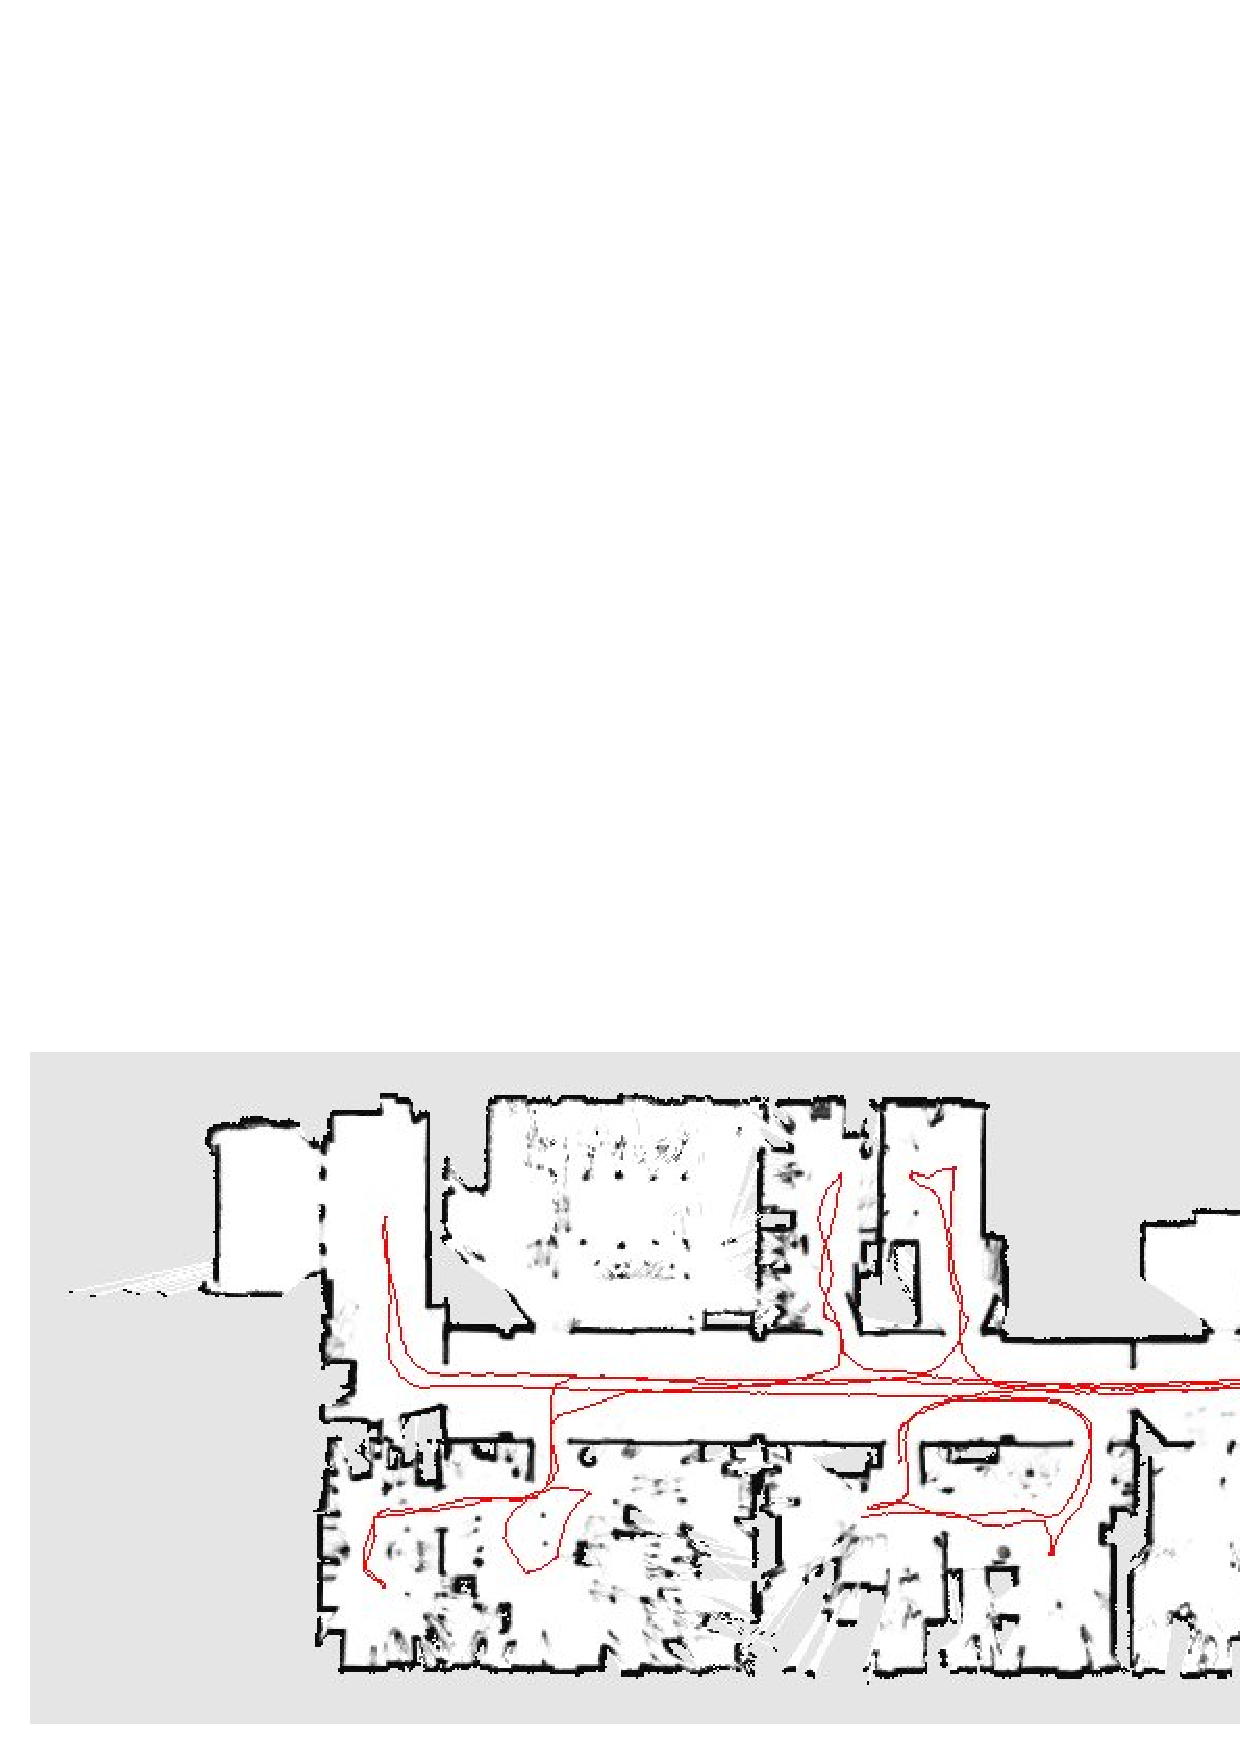
\includegraphics[width=1.05\columnwidth,keepaspectratio]{images/freiburg.JPG}
	 \caption{Example of a testing environment, University of Freiburg.  Image
	 was taken from RADISH, \cite{Radish}}
	\end{figure}
\end{frame}

\subsection*{Runtime Comparision}
\begin{frame}
\frametitle<1>{Runtime Comparision (Core 2 Duo)}
\frametitle<2>{Runtime Comparision (Coppermine)}
\transfade%\transdissolve
\pgfbox[center,center]{ 
        \begin{tikzpicture}[overlay,line width = 0.1cm, blue] 
		\node[color=blue,anchor=east, rotate=90] at (0.7,-1.3) (arrow_label) {better};
          \draw[->] (1,0) -- (1,-4); 
        \end{tikzpicture} 
      }
	\vspace{-10pt}
	\begin{figure}
	 \centering
	 %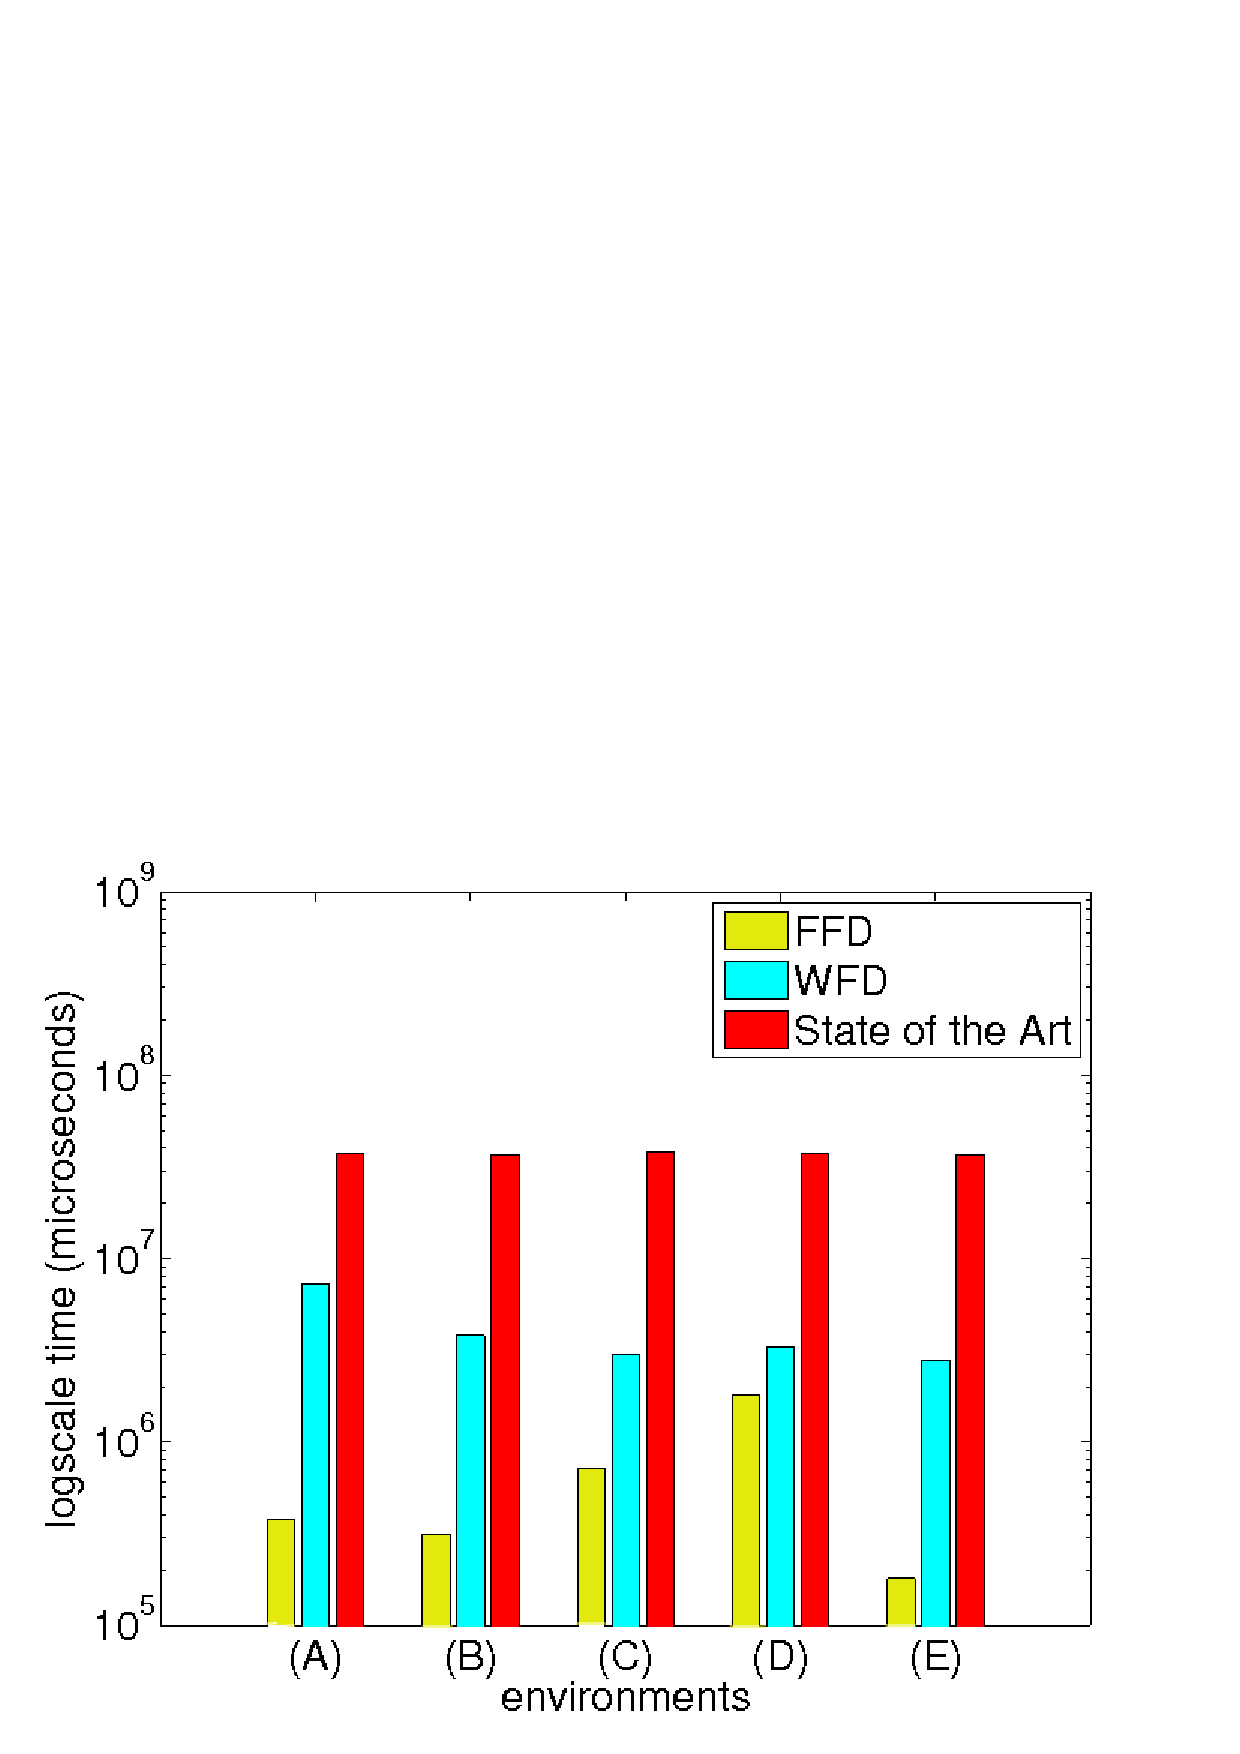
\includegraphics[width=0.65\columnwidth,keepaspectratio]{images/graph_Results_core2_yellow.pdf}
	 \includegraphics<1>[width=0.7\textwidth,keepaspectratio,angle=0]{../Thesis/graphs/plot_Results_five_algorithms.pdf}
	 \includegraphics<2>[width=0.7\textwidth,keepaspectratio,angle=0]{../Thesis/graphs/plot_Results_coppermine.pdf}
	\end{figure}
	\vspace{-10pt}
	\begin{itemize} 
  \item Y axis: mean execution time (microseconds) on a \emph{logaritmic scale} 
  \item \WFD,\WFDINC: faster than \SOTA by an order of magnitude 
  \item \FFD,\WFDIP: faster than \SOTA by two orders of magnitude 
\end{itemize}
\end{frame}

\begin{frame}
\frametitle{What Happend in Environment (D)?}

\begin{alertblock}{What Happend?}
	The mean run-time of \WFD is not relatively slower than \FFD
\end{alertblock}
\pause
\begin{exampleblock}{Answer}
	\begin{itemize}
	  \item Environment (D) contains regions that contains small obstacles
	  \item The obstacles enlarge the length of contour scanned by \FFD
	  \item As shown, the contour length affects the run-time complexity
	\end{itemize}
\end{exampleblock}

\begin{figure} 
 \centering
 \visible<2>{\includegraphics[width=0.25\columnwidth,keepaspectratio,angle=0]
 {../Thesis/images/environment_D_bad_contour_example2.pdf}}
\end{figure}

\end{frame}

\begin{frame}
\frametitle{Why is \WFDINC Sometimes Worse than \WFD?}

\begin{alertblock}{What Happend?}
	\begin{itemize}
	  \item In the worst-case, \WFDINC should perform the same as \WFD
		%\begin{itemize}
		%  \item Including an overhead of maintenance
		%\end{itemize}
	  \item The run-time means of \WFD and \WFDINC do not have a trend
	\end{itemize}
\end{alertblock}
\pause
\begin{exampleblock}{Hypothesis}
	\begin{itemize}
	  \item Certain environments have high frequency of particle
	  change
	  \item $\Rightarrow$ \WFDINC cleans its previous detected frontiers more often
	  
	\end{itemize}
\end{exampleblock}

\begin{table}
\centering
\begin{tabular}{|c|c|c||c|}
\hline \textbf{Map}&\textbf{Changes}&\textbf{Executions}&\textbf{Percent (\%)}
\\
\hline 
\hline (A)& 56 & 110 & 50.91  \\
\hline (B)& 52 & 287 & 18.12  \\
\hline (C)& 25 & 160 & 15.62  \\
\hline (D)& 193 & 429 & 44.99 \\ 
\hline (E)& 73 & 340 & 21.47 \\ \hline
\end{tabular}
\end{table}

\end{frame}

% \begin{frame}
% \frametitle{What Happend to \WFDIP in Environments (A),(C),(E), Weak Machine?}
% \begin{itemize}
%   \item Strong machine: \WFDIP outperforms all other algorithms
%   \item Weak machine: the situation is different in maps (A),(C),(E) \pause
%   \item Hypothesis (1) Memory: 
% 		\begin{itemize}
% 		  \item Weak machine is equipped with less RAM than strong machine
% 		  \item \WFDIP holds a separate instance of \WFDINC for each particle 
% 		  \item Hypothesis: strong machine runs each thread on a separate core
% 		  \item In our experiment, 30 instances of \WFDINC
% 		\end{itemize} \pause
%   \item Hypothesis (2) CPU: 
% 		\begin{itemize}
% 		  \item Weak machine is equipped a single CPU
% 		  \item GMapping runs two threads (Main thread and SLAM thread)
% 		  \item Hypothesis: strong machine runs each thread on a separate core  
% 		\end{itemize} 
% \end{itemize}
% \end{frame}

\subsection*{Evaluating FFD in a Finer Resolution}
\begin{frame}
\frametitle{Measuring Run-Time for Individual Particle}
\only<1>{
\begin{itemize}
  \item Particle-filter: each hypothesis runs its own instance of \FFD
  \item Investigate \FFD in a finer resolution
  \item Compare run-time of individual particles in each map
  %\item Each bar represents a specific particle
  %\item Vertical axis: measures the run-time of \FFD for the particle
  %\item Error-bars: the standard deviation of each particle's run-time
  
\end{itemize}
}
\only<2>{

\begin{figure}[htp]
%\vspace{-60pt}
 \centering 
 \subfigure[] {
 \centering
 \includegraphics[width=0.31\columnwidth,keepaspectratio]{../Thesis/graphs/graph_particle_times_ubremen-cartesium-demo2.pdf}
 }
 \subfigure[] {
 \centering
 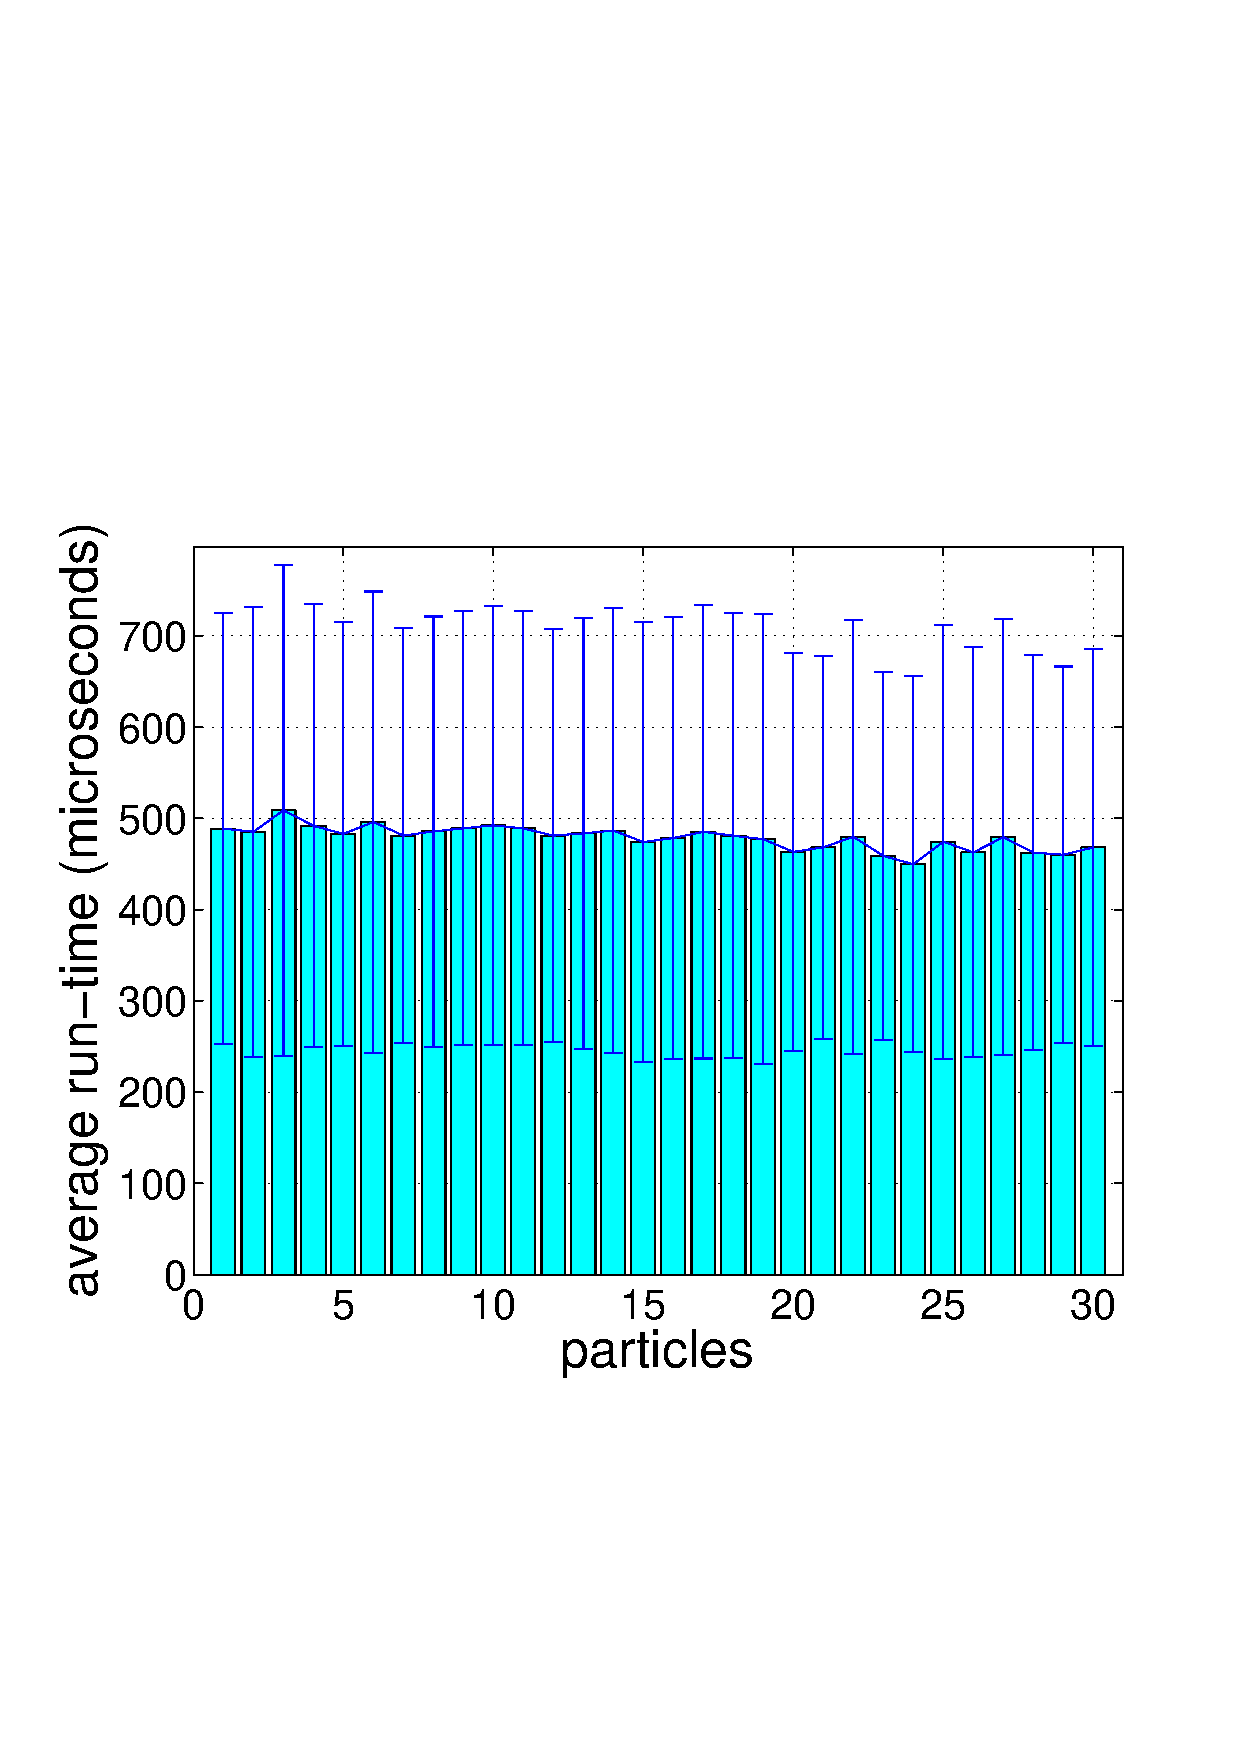
\includegraphics[width=0.31\columnwidth,keepaspectratio]{../Thesis/graphs/graph_particle_times_fr079-sm.pdf}
 }
 \subfigure[] {
 \centering
 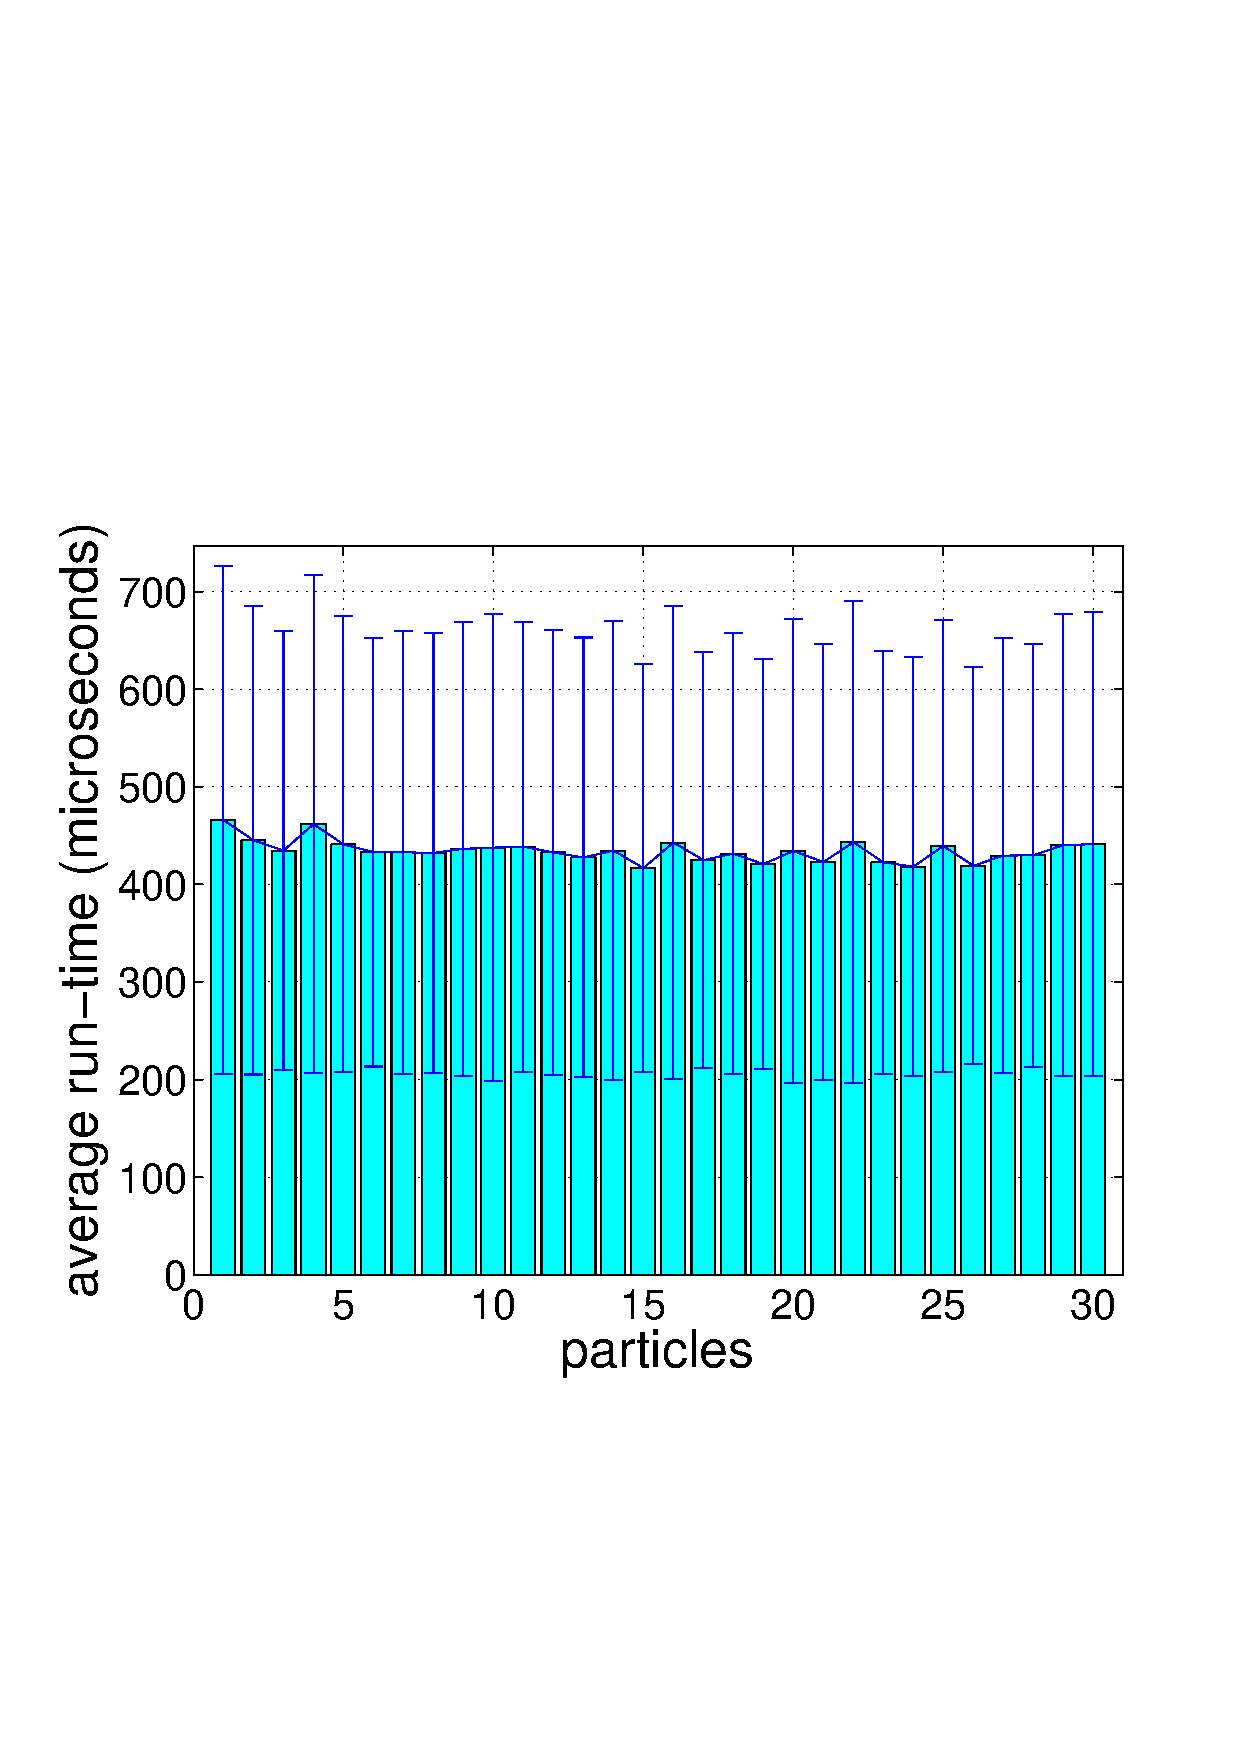
\includegraphics[width=0.31\columnwidth,keepaspectratio]{../Thesis/graphs/graph_particle_times_fr-campus-20040714.pdf}
 }
 \subfigure[] {
 \centering
 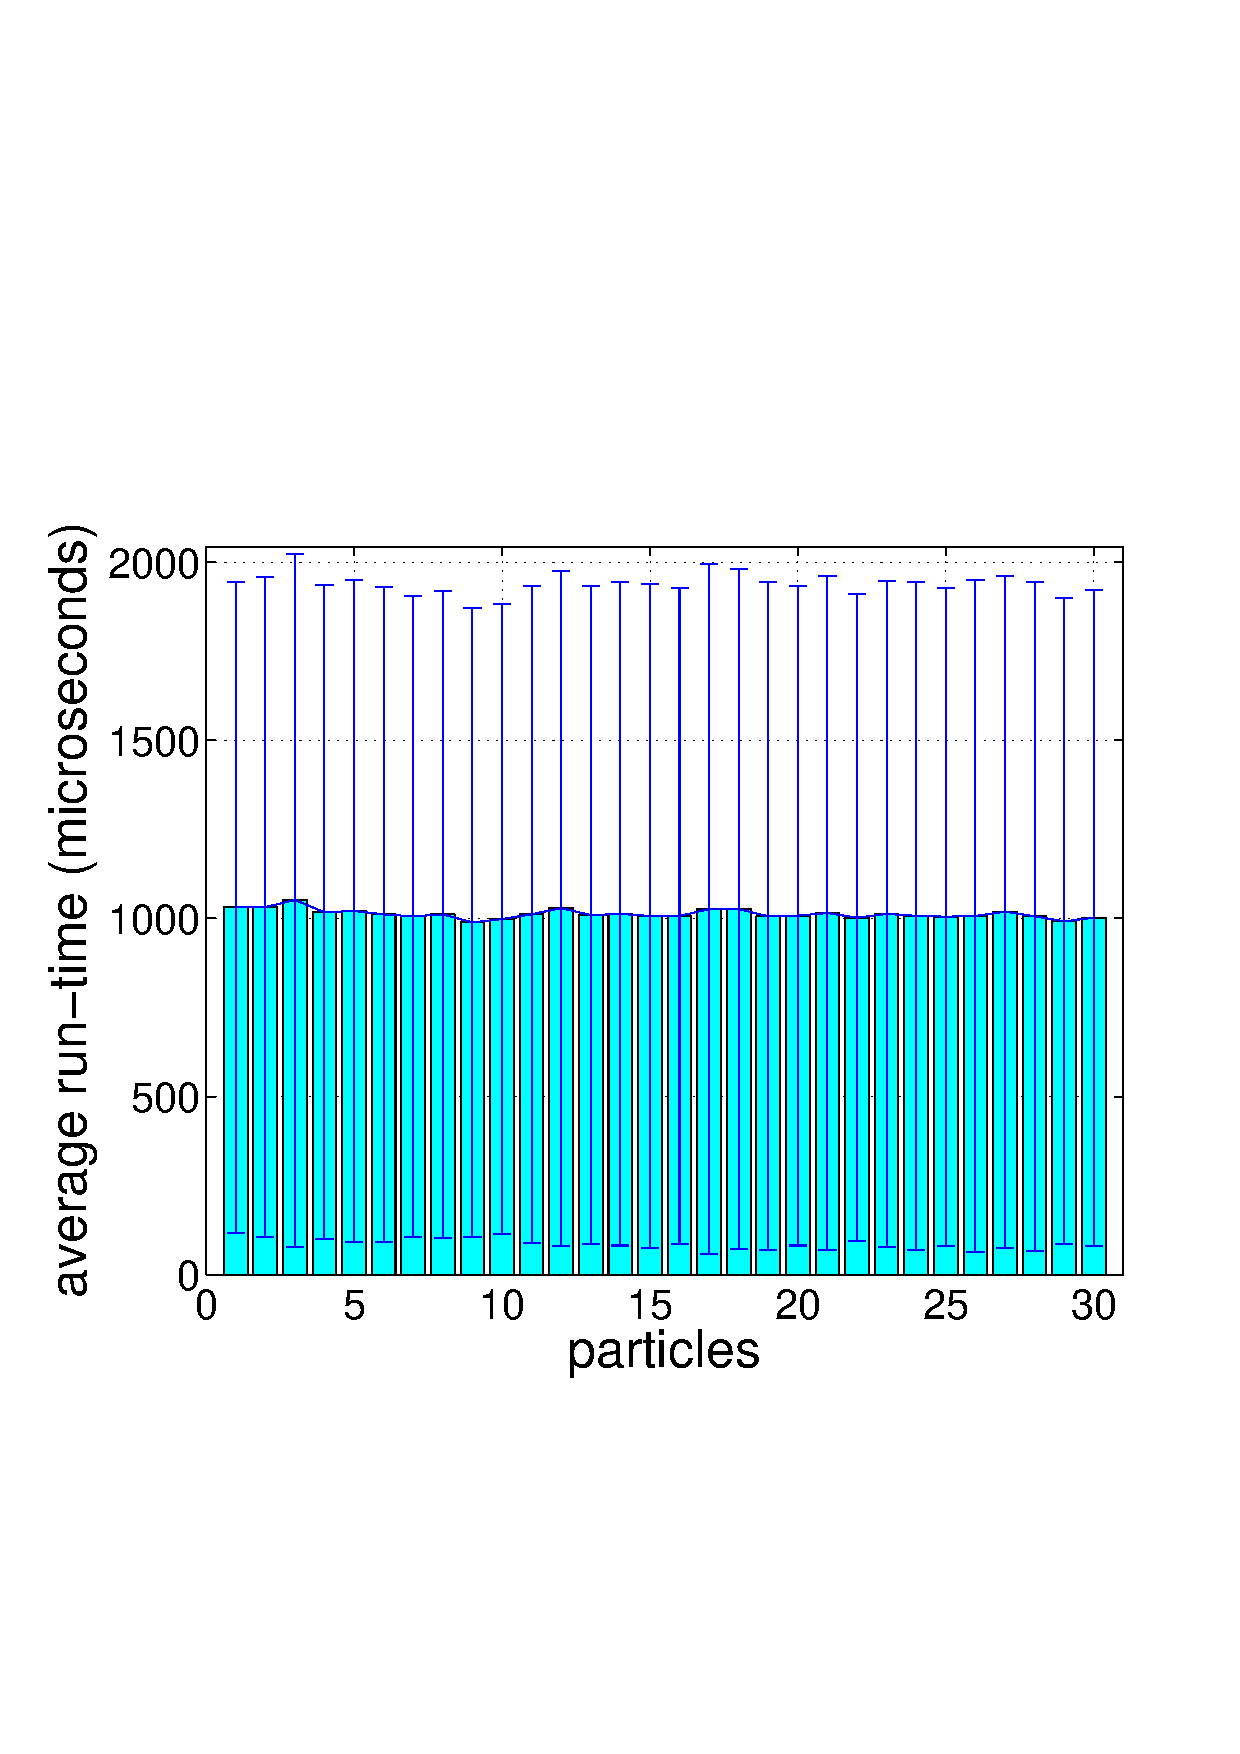
\includegraphics[width=0.31\columnwidth,keepaspectratio]{../Thesis/graphs/graph_particle_times_mit-csail-3rd-floor-2005-12-17-run4.pdf}
 }
 \subfigure[] {
 \centering
 \includegraphics[width=0.31\columnwidth,keepaspectratio]{../Thesis/graphs/graph_particle_times_edmonton_3.pdf}
 }
\end{figure}
}
\end{frame}

\begin{frame}
\frametitle{\FFD Performance According to Number of Particles}
\only<1>{
\begin{itemize}
  %\item \FFD has to persistently run in the background
  %\item Particle-filter systems: each particle has its own instance of \FFD
  %\item Hence, the overall run-time is increased \pause
  \item Investigate how number of particles affects on \FFD performance 
  \item We change the number of particles in different maps
  \item Measure how overall run-time is increased
  %\item Each bar represents a run with a specific number of particles
  %\item Vertical axis: mean run-time of \FFD for the configuration
  %\item Error-bars: standard deviation of each configuration run-time
\end{itemize}
}
\only<2>{
\setcounter{subfigure}{0}
\begin{figure}
 \centering 
 \subfigure[] {
 \centering
 \includegraphics[width=0.31\columnwidth,keepaspectratio]{../Thesis/graphs/plot_ubremen-cartesium-demo2_gfs_log_Particles.pdf}
 }
 \subfigure[] {
 \centering
 \includegraphics[width=0.31\columnwidth,keepaspectratio]{../Thesis/graphs/plot_fr079-sm_log_Particles.pdf}
 }
 \subfigure[] {
 \centering
 \includegraphics[width=0.31\columnwidth,keepaspectratio]{../Thesis/graphs/plot_fr-campus-20040714_carmen_log_Particles.pdf}
 }
 \subfigure[] {
 \centering
 \includegraphics[width=0.31\columnwidth,keepaspectratio]{../Thesis/graphs/plot_mit-csail-3rd-floor-2005-12-17-run4_flaser_log_Particles.pdf}
 }
 \subfigure[] {
 \centering
 \includegraphics[width=0.31\columnwidth,keepaspectratio]{../Thesis/graphs/plot_edmonton_3_log_Particles.pdf}
 }
\end{figure}
}
\end{frame}

% \begin{frame}
% \frametitle{Results}
% \begin{itemize}
%   \item Each group of bars represents run in a specific environment 
%   \item Y axis measures the average execution time (microseconds)
%   	\begin{itemize}
%   	  \item on a \emph{logaritmic scale}
%     \end{itemize} 
%   \item \WFD is faster than \SOTA by two orders of magnitude 
%   \item \FFD is faster than \WFD by an order of magnitude 
% \end{itemize}
% \end{frame}

\section{Conclusions and Future Work}
\label{chap:conclusions}
\section{Summary}

% \begin{frame}<beamer>
% \frametitle{Outline}
% \tableofcontents[currentsection,currentsubsection]
% \end{frame}

\begin{frame}<beamer>
\frametitle{Summary and Future Work}
\begin{itemize}
  \item Frontier Detection: a problem ignored by others 
  %\item Reducing frontier detection time can reduce exploration time
  \item \WFD, \FFD, \WFDINC, \WFDIP: methods for frontier detection
%   		\begin{itemize}
%   		  \item significant reduction of calculation time
%   		\end{itemize}
  \item Complexity and Correctness Analysis
  \item Reduction of 1--2 orders of magnitude of run-time
  		\begin{itemize}
  		  \item Fastest algorithm in the world!
  		\end{itemize}
  \item Theoretical and empirical results 
  \item Result: real-time frontier detection on weak CPU's
  \item Publications:
  	\begin{itemize}
  	  \item AAMAS 2012
  	  \item ARMS workshop at AAMAS 2011 
  	\end{itemize}
  \item Future work:
  	\begin{itemize}
	  \item Address efficient methods for maintaining frontiers in \FFD
	  %\item Integrate \FFD into EKF-based systems
	  \item Novel exploration policies based on real-time
	  frontier-detection
	\end{itemize}
%   \item {For more information:}
%   	\begin{itemize}
%   	  \item \url{matankdr@gmail.com}
%   	  %\item \email{eranpolo@gmail.com}
%   	  \item \url{galk@cs.biu.ac.il}
%     \end{itemize}
\end{itemize}
\end{frame}

\bibliographystyle{abbrv}
\bibliography{full,ffd_bib}
\end{document}
